\chapter{Grandeurs\\et mesures} \label{Grm7}

\begin{prerequis}[Les attendus des enfants en fin d'école maternelle]
{\bf Explorer des grandeurs}
   \begin{itemize}
      \item Classer ou ranger des objets selon un critère de longueur ou de masse ou de contenance.
   \end{itemize}
\end{prerequis}

\begin{prerequis}[Dans les programmes - cycle 2]
      {\bf\small Comparer, estimer, mesurer des longueurs, des masses, des contenances, des durées. Utiliser le lexique, les unités, les instruments de mesures spécifiques à ces grandeurs}
   \begin{itemize}
      \item Comparer des objets selon plusieurs grandeurs et identifier quand il s’agit d’une longueur, d’une masse, d’une contenance ou d’une durée.
      \item Comparer des longueurs, des masses et des contenances, directement, en introduisant la comparaison à un objet intermédiaire ou par mesurage.
      \item Estimer à vue des rapports très simples de longueur.
      \item Estimer les ordres de grandeurs de quelques longueurs, masses et contenances en relation avec les unités métriques. Vérifier avec un instrument dans les cas simples.
      \item Dans des cas simples, mesurer des longueurs, des masses et des contenances en reportant une unité et en utilisant un instrument adapté
      \item Encadrer une grandeur par deux nombres entiers d’unités. 
      \item Lire l’heure sur une horloge ou une montre à aiguilles.
      \item Comparer, estimer, mesurer des durées.
      \item Dans des cas simples, représenter une grandeur par une longueur, notamment sur une demi-droite graduée.
      \item Lire les graduations représentant des grandeurs : cadran d’une balance, thermomètre, frise chronologique, axes d’un graphique gradués en unités.
   \end{itemize}
\end{prerequis}

\begin{prerequis}[Dans les programmes - cycle 3]
   {\bf\small Comparer, estimer, mesurer des grandeurs géométriques avec des nombres entiers et des nombres décimaux : longueur, aire, volume, angle. Utiliser le lexique, les unités, les instruments de mesures spécifiques de ces grandeurs}
   \begin{itemize}
      \item Longueur et périmètre : comparer des périmètres avec ou sans recours à la mesure ; calculer le périmètre d’un polygone, d’un carré et d’un rectangle, la longueur d’un cercle, en utilisant ou non une formule.
      \item Aires : comparer des surfaces selon leurs aires sans avoir recours à la mesure ; différencier périmètre et aire d’une figure ; estimer la mesure d’une aire et l’exprimer dans une unité adaptée ; déterminer la mesure de l’aire d’une surface à partir d’un pavage simple ou en utilisant une formule.
      \item Volumes et contenances : relier les unités de volume et de contenance ; estimer la mesure d’un volume ou d’une contenance par différentes procédures et l’exprimer dans une unité adaptée ; déterminer le volume d’un pavé droit en se rapportant à un dénombrement d’unités.
      \item Angles : identifier des angles dans une figure géométrique ; comparer des angles sans avoir recours à leur mesure ; reproduire un angle donné en utilisant un gabarit ; estimer qu’un angle est droit, aigu ou obtus ; utiliser l’équerre pour vérifier qu’un angle est droit, aigu ou obtus, ou pour construire un angle droit.
   \end{itemize}
\end{prerequis}


\reperes

%%%%%%%%%%%%%%%%%%%%%%%%
\section{Progressivité des apprentissages} % 2.B

La question \og qu’est-ce qui est le plus lourd : un kilo de plumes ou un kilo de plomb ? \fg{} posée en classe pourra permettre de débattre sur le vocabulaire et les conceptions des élèves. En effet, certains diront que c'est pareil puisque les deux pèsent 1 kg, mais certains élèves pourraient dire que les plumes pèsent plus parce qu'elles occupent plus de place, ou encore que c'est le plomb qui pèse le plus car le plomb est lourd alors que la plume est légère. 

Il est donc très important de commencer à travailler sur le concept de grandeur avant d'aborder la mesure. En effet, les confusions sont nombreuses chez les élèves, par exemple entre aire et périmètre ou masse et volume. Il est indispensable de manipuler les grandeurs sans mesures : les comparer directement, à l'aide d'un objet intermédiaire ou par transformations. C'est seulement ensuite qu'ils apprennent à effectuer des mesures au moyen d’instruments adéquats en s’appropriant peu à peu les unités usuelles.

{\renewcommand{\StringDOCUMENTATION}{Démarche générale pour conceptualiser les grandeurs}
\begin{documentation}
   \begin{itemize}
      \item {\bf Comparer et ordonner des grandeurs sans mesurer par comparaison directe} : la comparaison des grandeurs peut s’effectuer dans un premier temps à partir de manipulations d’objets, par comparaison directe (perception, juxtaposition, superposition, souspesage\dots). Cette étape est essentielle car elle permet de donner du sens à la grandeur.
      \item {\bf Comparer et ordonner des grandeurs sans mesurer par comparaison indirecte} : la comparaison se fait grâce à un objet intermédiaire (balance, ficelle, bande de papier, transvasage, découpage\dots) pour des objets qui ne permettent pas la comparaison directe, c'est-à-dire non déplaçables ni superposables, pas présents en même temps.
      \item {\bf Comparer et ordonner des grandeurs en les mesurant grâce à un étalon} : cette étape nait d'un besoin de communication, pouvoir écrire le résultat de notre mesure nécessite une unité commune appelée étalon.
      \item {\bf Découvrir des unités et mesurer des grandeurs} : les unités que l’on étudie à l’école appartiennent au SI, elles sont le résultat d’un choix arbitraire qui permet de mesurer grâce à des unités connues de tous. Cette étape permet d'introduire les multiples/sous-multiples.
      \item {\bf Effectuer des calculs et des changements d’unités} : le mesurage n'est plus nécéssaire, les données sont fournies et il s'agit de les utiliser de manière directe. On effectue des conversions entretenant ainsi l'articulation entre la numération, le système métrique et les situations de la vie courante ainsi que celle entre les grandeurs/mesures et la géométrie. \\ [-8mm]
   \end{itemize}
\end{documentation}

\bigskip

Il sera très important, au moment de l'introduction de la mesure, d'insister sur la rédaction et sur la nécessité de bien indiquer les unités, y compris dans les calculs en ligne. Cela permet également de renforcer le sens des opérations lors de la résolution de problème, en différenciant des opérations mathématiques qui paraitraient identiques sans les unités.
   
\begin{exemple}
\ \\ [-10mm]
   \begin{enumerate}
      \item J’ai un baton de longueur \ucm{45}, et j’ai besoin de bâtonnets de \ucm{5}. Combien vais-je pouvoir en faire ?
      \item J’ai un baton de longueur \ucm{45}, et j’ai besoin de 5 bâtonnets de même longueur. Quelle sera la longueur d'un bâtonnet ?
   \end{enumerate}
\correction
\ \\ [-10mm]
   \begin{enumerate}
      \item Le problème se modélise par une division quotition : \\
      $\ucm{45} : \ucm{5} =9$. \\
      Je vais pouvoir faire 9 bâtonnets de \ucm{5}.
      \item Le problème se modélise par une division partition : \\
      $\ucm{45} \div 5 =\ucm{9}$. \\
      Un bâtonnet mesurera \ucm{9}.
   \end{enumerate}
   Ces deux écritures sont bien plus parlantes que l’écriture sans unité $45 \div 5 = 9$, où ce dont on parle n’est pas indiqué.
\end{exemple}

\bigskip


On peut résumer par un tableau synoptique la progression des apprentissages dans ce domaine en fonction des niveaux de classe comme précisé dans les repères de progression des programmes. \\
{\bf Les éléments en gras concernent la mesure} et les unités à introduire. Les opérations sur les grandeurs sont menées en lien avec l’avancée des opérations sur les nombres, de la connaissance des unités et des relations entre elles. \smallskip

\begin{center}
{\hautab{1.4}
\setlength{\tabcolsep}{2pt}
   \begin{CLtableau}{\linewidth}{7}{C{2}}
      \hline
      Grandeur & C1 & CP & CE1 & CE2 & CM1 & CM2 \\
      \hline
      Longueur & comparer, trier, classer, ranger & comparer, estimer, mesurer  \newline {\bf cm, m} & comparer, estimer, mesurer \newline {\bf cm, dm, m, km} & comparer, estimer, mesurer \newline {\bf mm, cm, dm, m, km} & comparer, mesurer des périmètres \newline {\bf polygone} & {\bf formule du carré, rectangle ; périmètre du polygone, } \\
      \hline
      Masse & comparer, trier, classer, ranger & comparer & comparer, mesurer \newline {\bf g, kg} & mesurer \newline {\bf g, kg, tonne} & \multicolumn{2}{c|}{} \\
      \hline
      Contenance & comparer, trier, classer, ranger & & comparer \newline {\bf L} & comparer, mesurer \newline {\bf cL, dL, L} & comparer, mesurer \newline {\bf 1L = (10 cm)$^3$} & comparer, mesurer \newline {\bf L, dL, cL, mL} \\
      \hline
      Durée & & lire, repérer la date \newline jour, semaine, mois \newline lire l'heure entière (analogique) & lire l'heure, \newline la demi-heure (analogique) \newline {\bf j, h, min} & lire h, demi-h, \newline (analogique) \newline lire, donner h et min (numérique) \newline {\bf s, min, an, siècle, millénaire} & lire l'heure ; siècle/années, semaine/jours, h/min, min/s \newline {\bf calcul de durées et d'instants} & {\bf relations entre unités, \newline conversions} \\
      \hline
      Prix & & manipuler \newline {\bf pièces de 1\euro{}, 2\euro{}, billets de 5\euro{}, 10\euro{}, 20\euro{}, 50\euro{}, 100\euro{}} & \multicolumn{2}{c|}{\bf euro et centimes d'euro} & \multicolumn{2}{c|}{} \\
      \hline
      Aire & \multicolumn{4}{c|}{} & comparer, estimer, mesurer \newline {\bf aire avec étalon} & {\bf cm$^2$, dm$^2$, m$^2$ \newline formule du carré, rectangle, \newline triangle rectangle} \\
      \hline
      Angles & \multicolumn{4}{c|}{} & \multicolumn{2}{C{4.5}|}{repérer, comparer, estimer (gabarit) \newline angle droit, aigu, obtus} \\
      \hline
   \end{CLtableau}
}
\end{center}


\subsection{Les longueurs} %%%

{\bf -- Au C1}, les enfants distinguent les longueurs par des observations, des comparaisons (souvent directes), des tris. \\
{\bf -- Au CP}, les élèves comparent des objets, des segments (de manière directe et indirecte à l'aide ficelle ou de bandes de papier) selon leur longueur, d’abord en les estimant. Ils donnent du sens aux expressions \og plus long que \fg, \og plus court que \fg, \og aussi long que \fg, \og moins long que \fg, et aussi \og double \fg{} et \og moitié \fg. \\
   Ils mesurent des segments en utilisant des unités de référence puis en utilisant la règle graduée pour des mesures en centimètres entiers. Ils appréhendent le mètre (100 cm) à travers par exemple la règle du professeur. \\ 
{\bf -- Au CE1}, les élèves consolident les comparaisons, les estimations et les mesures de longueur en cm. Puis le travail se poursuit en utilisant les unités m, dm et km. Ces unités sont mises en relation. \\
{\bf -- Au CE2}, les élèves consolident les comparaisons, les estimations et les mesures de longueur en cm, m, dm et km. Le travail se poursuit en utilisant le mm et ils mettent les unités m, dm, cm et mm. \\
{\bf -- Au CM1}, les élèves comparent des périmètres d'abord sans mesure, puis par report d’unités, de fractions d’unités ou des longueurs des côtés sur un segment de droite avec le compas. Ils calculent le périmètre d’un polygone en ajoutant les longueurs de ses côtés (avec des entiers et fractions puis avec des décimaux à deux décimales). \\
{\bf -- Au CM2}, les élèves établissent les formules du périmètre du carré et du rectangle. \medskip

Les {\bf mots} du domaine des longueurs sont nombreux : hauteur, altitude, profondeur, taille, distance, largeur d’un rectangle, périmètre, circonférence\dots{} Il est important que tous ces mots, utilisés dans des contextes différents, se réfèrent au même concept, appelé en mathématiques \og longueur \fg. \medskip

Les {\bf instruments} qui peuvent être utilisés sont la règle graduée (d'écolier ou du tableau), des bandes de papier plus ou moins longues, de la ficelle, le pied à coulisse\dots{} La règle, utilisée jusque là comme instrument de géométrie pour tracer des ligne droites devient un instrument de mesure de longueurs par l'adjonction d'une graduation.  \medskip

{\hautab{1.1}
\begin{Ltableau}{\linewidth}{2}{p{6cm}|p{10cm}}
   \hline
   {\bf Compétences} & {\bf Difficultés} \\
   \hline
   Comparer, ordonner des longueurs : par superposition ; en utilisant un objet intermédiaire ou une unité de longueur
   &
   -- Élèves \og non conservants \fg{} : incapacité de repérer des transformations (déplacement, déformation\dots) \newline
   -- Difficultés de manipulation \\
   \hline
   Mesurer des longueurs
   &
   -- Erreurs liées au positionnement de l'instrument (\og 0 \fg{} d'un règle graduée, lecture des millimètres) \\
   \hline
   Estimer la longueur d'un objet
   &
   -- Par manque d'expériences sociales ou scolaires, l'élève n'a aucune idée des mesures de certaines longueurs \\
   \hline
   Effectuer des conversions d'unités
   &
   -- Erreurs liées à l'écriture décimale des nombres ou à la méconnaissance des relations entre les différentes unités. \\
   \hline
   Calculer le périmètre d'une figure
   &
   -- L'élève a une représentation du périmètre comme étant le résultat obtenu par un calcul à partir d'une formule \newline
   -- L'élève pense que pour calculer un périmètre il faut ajouter toutes les dimensions qui lui sont données \\
   \hline
\end{Ltableau}} \medskip

Afin d'accroître la difficulté ou, au contraire, de faciliter la compréhension des situation caractérisant des longueurs, on peut utiliser les {\bf variables didactiques} suivantes : \\
-- nature des objets dont il faut comparer les longueurs ou le périmètre : objets ou figures plus ou moins simples ; \\
-- taille de ces objets ou de la figure ; \\
-- objets déplaçables ou non, transformables ou non ; \\
-- matériel dont dispose l'élève : règle graduée ou non, bande, compas, ficelle\dots \\
-- support de la figure : quadrillage ou non, mesures données ou non.


\subsection{Les masses} %%%

{\bf -- Au C1}, les enfants sont amenés à distinguer les masses par des observations, des comparaisons, des tris. Les premières expériences sensitives permettent de travailler sur le vocabulaire \og lourd/léger \fg, à différencier de \og gros/petit \fg. \\
{\bf -- Au CP}, les élèves comparent des objets selon leur masse, en les soupesant puis en utilisant la balance à plateaux, type Roberval, sans que des unités de mesure soient nécessairement introduites. Ils donnent du sens aux expressions : \og Plus lourd que \fg, \og plus léger \fg\dots \\
{\bf -- Au CE1}, les élèves consolident les comparaisons d’objets selon leur masse. Ils mesurent des masses exprimées en g et kg et mettent en relations ces unités. Le trombone est un bon étalon \og non usuel \fg, pour les objets légers (1 g) et le paquet de farine pour des objets plus lourds, de l'ordre du kg, correspondant également à 1 000 trombones. \\
{\bf -- Au CE2}, les élèves consolident les mesures de masses d’objets (g et kg). Ils utilisent l’unité tonne (t) et mettent en relations les unités g, kg et kg, t.  \medskip

 Traditionnellement, à l'école, comme dans le langage courant, on confond masse d'un objet et poids de cet objet. La compréhension du {\bf sens propre et du sens figuré} est une compétence à développer chez les élèves pour leur permettre d’accéder à une compréhension fine des textes. En effet, dans le langage commun, de multiples expressions font appel à ce concept : se fondre dans la masse, s'écrouler comme une masse, faire pencher la balance de son côté, avoir le c\oe ur léger ou la main lourde\dots \medskip
   
   Les {\bf outils} de comparaison et de mesure ne sont pas des instruments d'écolier classiques. On pourra utiliser une balance de Roberval\footnote{Gilles Personne de Roberval (1602-1675) est un mathématicien et physicien français, inventeur de la balance à fléaux qui porte son nom.} ou à plateaux dans un premier temps, puis une balance numérique. L'avantage des balances mécaniques, c'est qu'elles permettent de comparer et de mesurer selon l'usage que l'on en fait. 
\begin{center}
   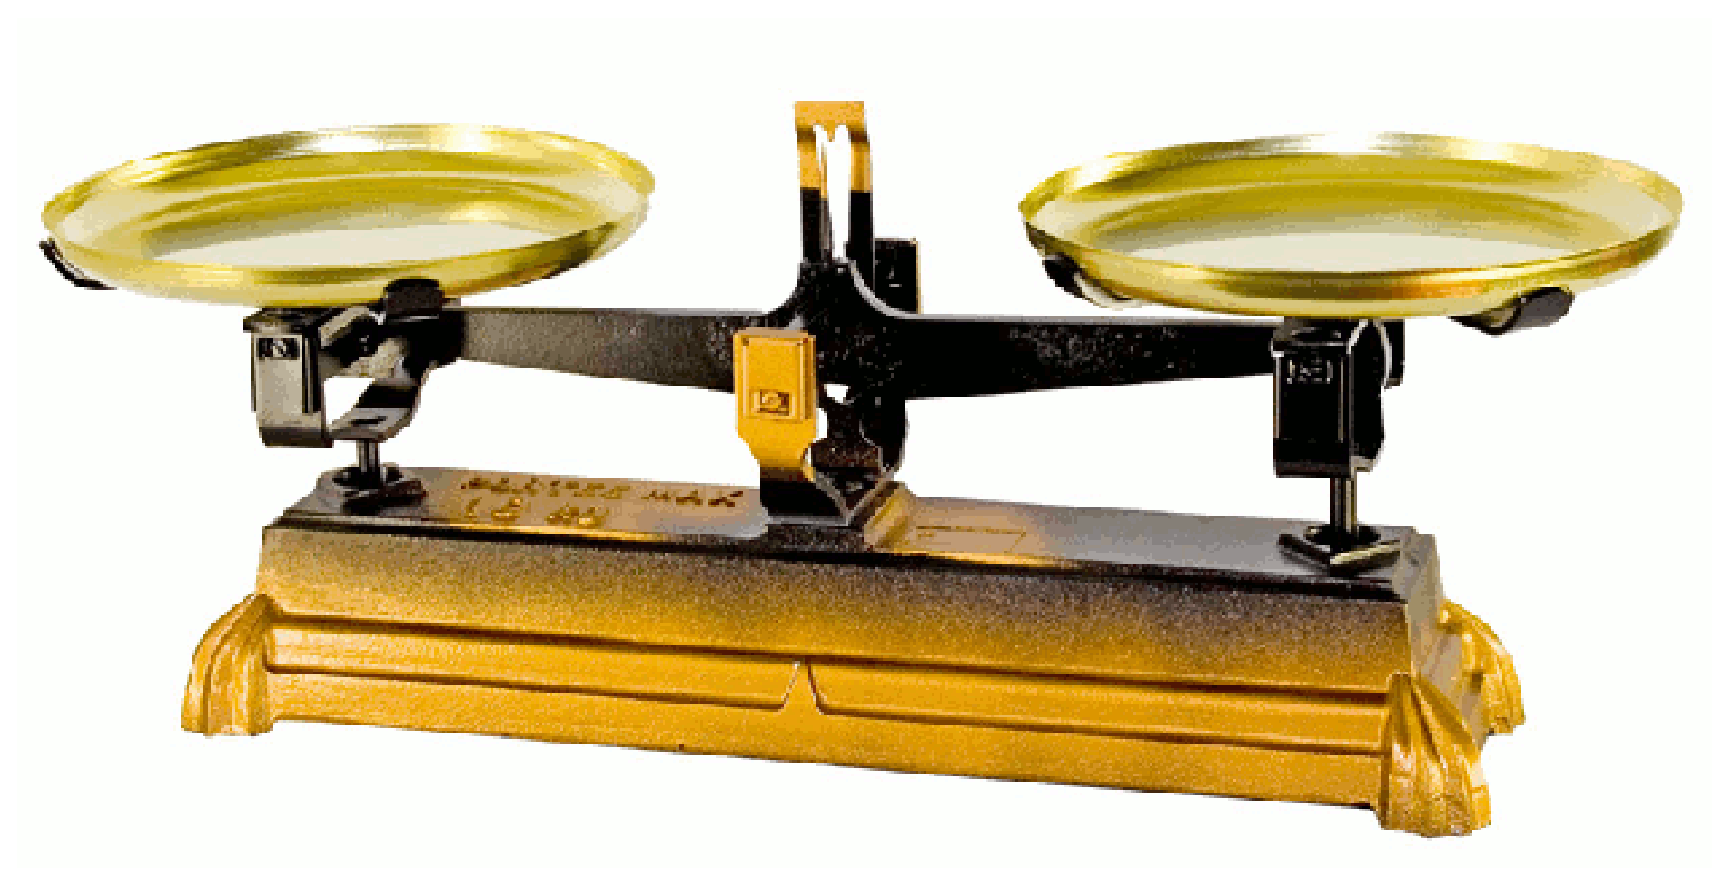
\includegraphics[width=5.5cm]{Grandeurs_mesures_did/Images/Grm7_cours_Robervall}
   \quad
   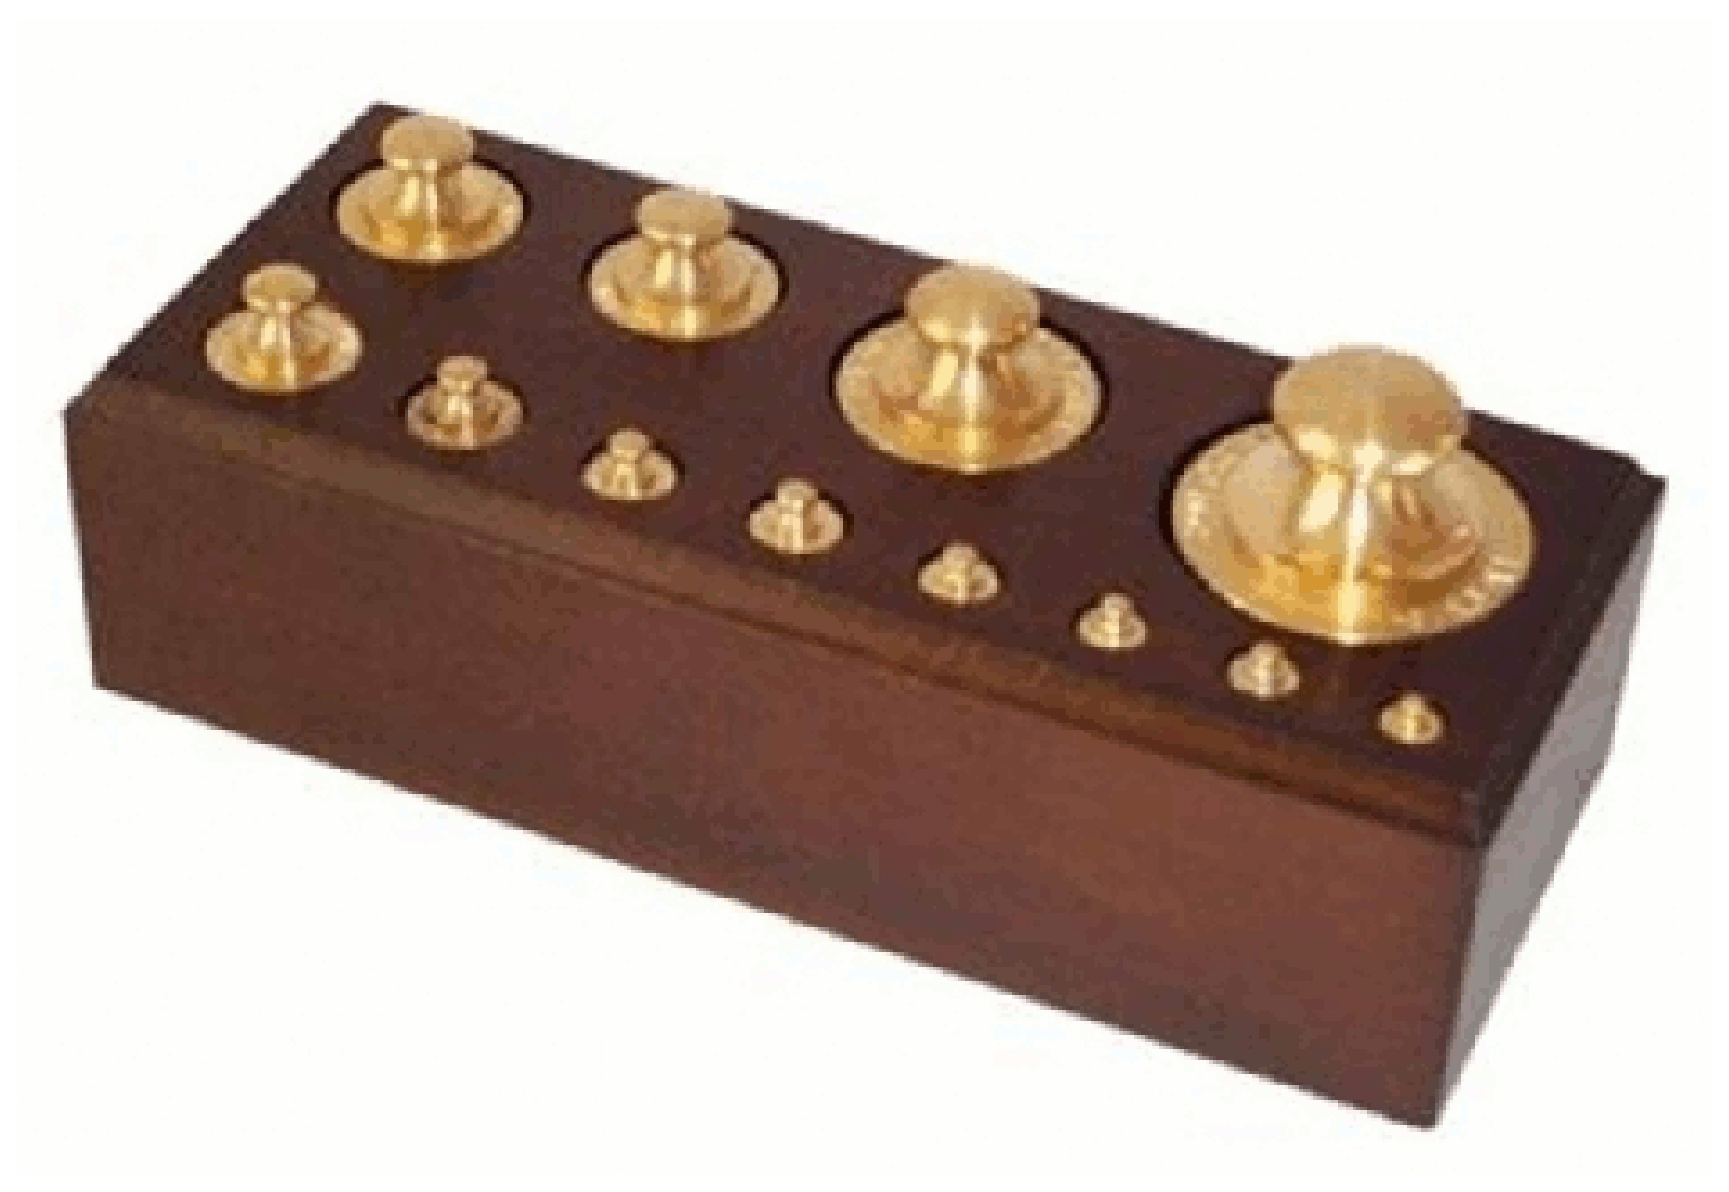
\includegraphics[width=3cm]{Grandeurs_mesures_did/Images/Grm7_cours_poids}
   \qquad
   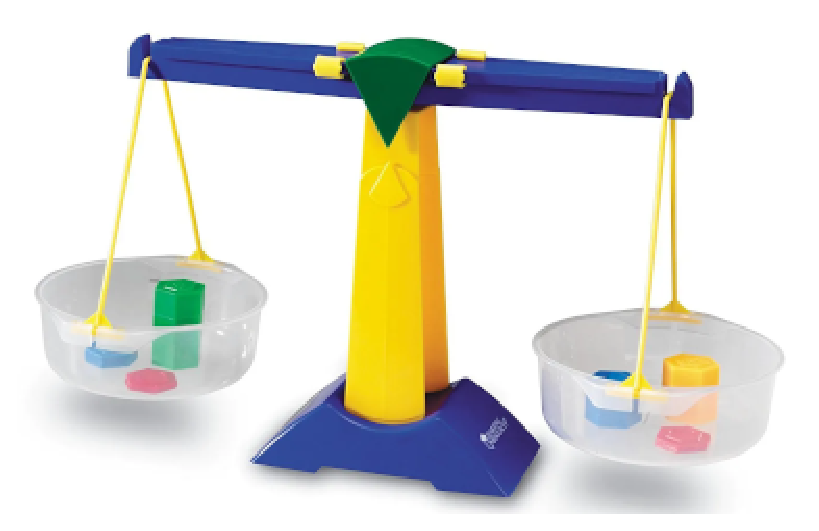
\includegraphics[width=5cm]{Grandeurs_mesures_did/Images/Grm7_cours_balance_plateaux}
\end{center}
Outre les difficultés de conversion, les élèves ont du mal à estimer le poids de certains objets, par exemple parce qu'ils n'ont pas idée de ce que représentent le gramme ou le kilogramme, d'où la nécessité de faire manipuler des objets, mais aussi parce que ces objets ne leur sont pas familiers, ou très lourds et donc non \og portables \fg.

\begin{center}
   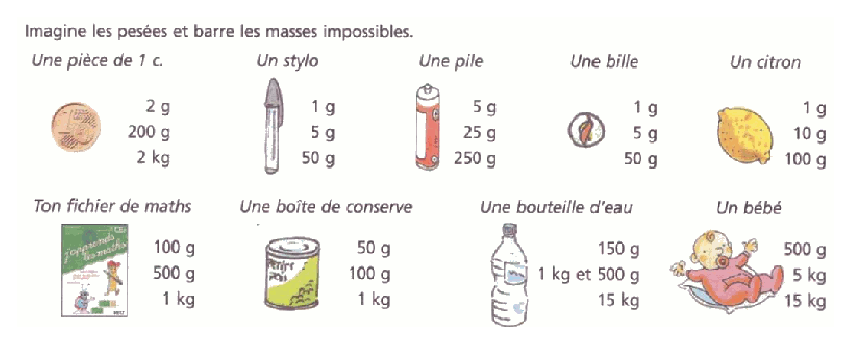
\includegraphics[width=15cm]{Grandeurs_mesures_did/Images/Grm7_cours_masses}
\end{center}


\subsection{Les contenances} %%%

{\bf -- Au C1}, les enfants sont amenés à distinguer les contenances par des observations, des comparaisons, des tris. Ils travailent sur le vocabulaire \og gros/petit \fg, à différencier de \og lourd, léger \fg, en lien avec les masses. \\
{\bf -- Au CE1}, les élèves continuent à comparer des objets selon leur contenance, en les observant (comparer \og visuellement \fg{} différents récipients remplis d'eau) et en les manipulant. Il peuvent comparer les contenances de plusieurs bouteilles à l'aide d'un verre-étalon, puis les mesurer en \og verre-étalon \fg, par transvasement, et enfin ils découvrent que le litre (L) est une unité de contenance usuelle. \\
{\bf -- Au CE2}, les élèves comparent des objets selon leur contenance en utilisant le L. Ils utilisent le cL, dL et le L et connaissent leurs relations (par exemple à l'aide des gobelets de contenance \ucl{10} et d'une bouteille d'\ul{1}). \\
{\bf -- Au CM1}, Les élèves comparent des contenances sans les mesurer, puis en les mesurant. Ils découvrent et apprennent qu’un litre est la contenance d’un cube de 10 cm d’arête. Ils font des analogies avec les autres unités de mesure à l’appui des préfixes. \\
{\bf -- Au CM2}, les élèves poursuivent ce travail en utilisant de nouvelles unités de contenance : dL, cL et mL. \medskip

Usuellement, les volumes sont mesurés en \og {\bf unité cube} \fg{} qui vont de mille en mille. Cette mesure n’est pas adaptée pour les liquides utilisés dans la vie quotidienne (comme l’huile, l’eau, le lait par exemple). Les contenances, ou capacités -- dans la pratique, on parle en général de capacité pour les bouteilles et de contenance pour les autres récipients -- sont plutôt exprimées en {\bf litre}. Ce dernier a son équivalent en volume puisqu'une contenance d’un litre représente un volume d’un décimètre cube. On parle ainsi du volume d’un vase (\udmq{1} par exemple) mais on évoque la contenance de celui-ci en litre (\ul{1} par exemple). \\
En cycle 3, et en continuité avec le cycle 2, la notion de volume sera vue d’abord comme une contenance : les élèves découvrent et apprennent qu’un litre est la contenance d’un cube de \ucm{10} d’arête, mais la formalisation et le calcul de volumes ne se fera qu'à partir de la 6\up{e}.
\begin{center}
   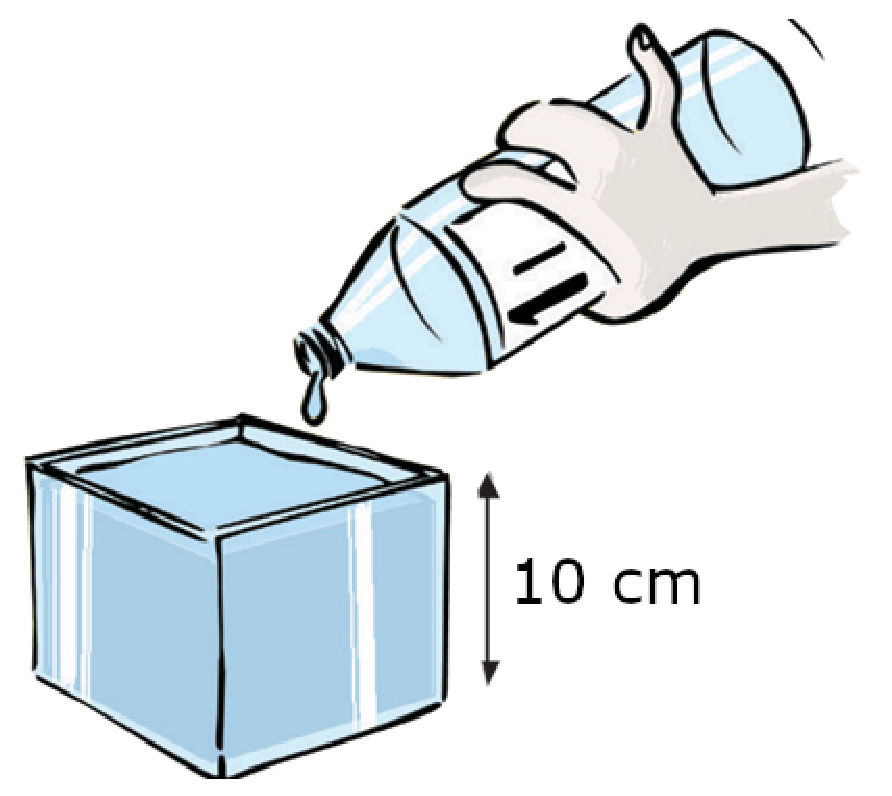
\includegraphics[width=4cm]{Grandeurs_mesures_did/Images/Grm7_cours_L_dm3}
   \qquad 
   {\psset{unit=0.7}
   \begin{pspicture}(-3,-0.25)(7,5.5)
      \rput(-2,2){{\huge $\Longrightarrow$}}
      \psline(0.5,0.5)(0.5,3.75) %bouteille
      \psline(2,0.5)(2,3.75)
      \psarc(1.5,3.75){0.5}{0}{90}
      \psarc(1,3.75){0.5}{90}{180}
      \psline(1,4.25)(1,5)
      \psline(1.5,4.25)(1.5,5)
      \psellipticarc(1.25,0.5)(0.75,0.3){180}{0}
      \psellipticarc(1.25,3.5)(0.75,0.3){180}{0}
      \psellipticarc[linestyle=dashed](1.25,3.5)(0.75,0.3){0}{180}
      \psellipse(1.25,5)(0.25,0.1)
      \rput(1.25,2){\textcolor{A1}{\ul{1}}}
      \rput(3,1.8){\Large$=$}
      \psframe(4,0.5)(6,2.5) %cube
      \psline(4,2.5)(4.75,3.25)(6.75,3.25)(6.75,1.25)(6,0.5)
      \psline(6,2.5)(6.75,3.25)
      \rput(5,0){\textcolor{A1}{$\udm{1} =\ucm{10}$}}
      \rput(5,1.5){\textcolor{A1}{$\udmc{1}$}}
   \end{pspicture}}
\end{center}
Tout comme les masses, il est important de faire découvrir quelques exemples de capacités usuelles. Les recettes de cuisine sont aussi un outil très pertinent pour travailler les contenances, ainsi que les masses et ainsi de faire différencier ces deux concepts. On fera remarquer que les préfixes utilisés pour les longueurs sont les mêmes et ont la même signification pour les masses et les contenances.

\begin{center}
   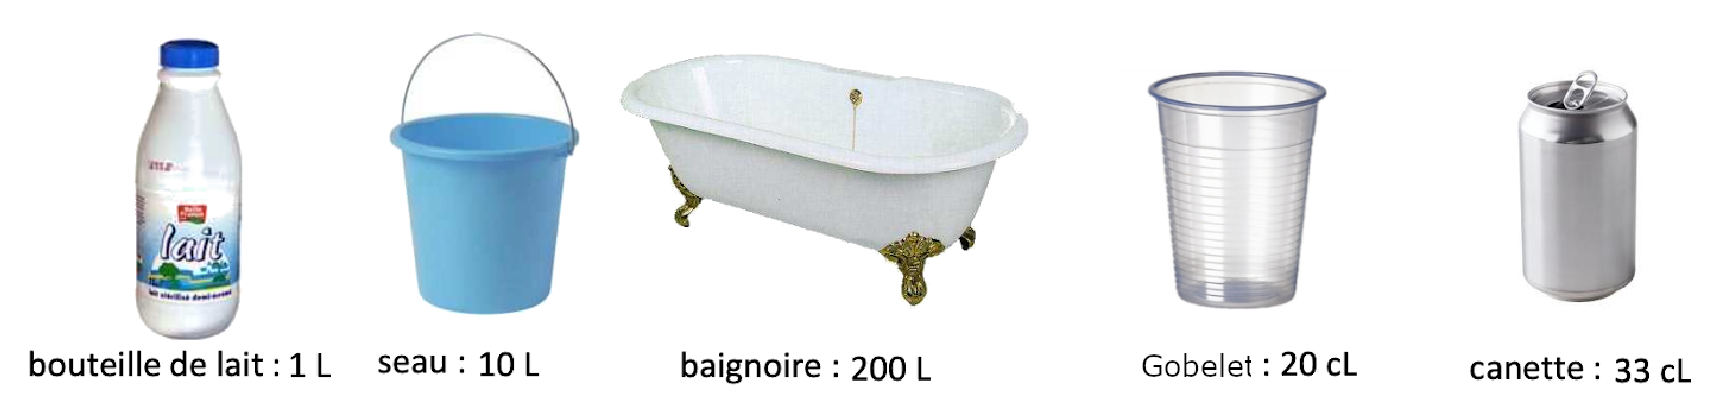
\includegraphics[width=17cm]{Grandeurs_mesures_did/Images/Grm7_cours_contenances}
\end{center}


\subsection{Les durées} %%%

{\bf -- Au CP}, les élèves apprennent à lire une date sur un calendrier et à se repérer dans celui-ci. Ils repèrent les jours et les semaines puis les mois ; ils mettent en relation jour et semaine. En lien avec le domaine \og questionner le monde \fg, ils apprennent à lire l’heure sur une horloge à aiguilles en heures entières. \\
{\bf -- Au CE1}, les élèves lisent les heures entières et les demi-heures sur une horloge à aiguilles. Ils mettent en relation les unités de durée h et min, ainsi que j et h. \\
{\bf -- Au CE2}, les élèves consolident la lecture de l’heure sur une horloge à aiguilles (heure entière et demi-heure). Ils lisent et donnent l’heure (exemple : \og quatre heures moins vingt \fg{} ou 15 h 40 ; \og sept heures et quart \fg{} ou 7 h 15). \\
Ils utilisent les unités année, siècle, millénaire et  min, s et connaissent leurs relations. \\
{\bf -- Au CM1}, les élèves consolident la lecture de l’heure et l’utilisation des unités de mesure des durées et de leurs relations ; des conversions peuvent être nécessaires (siècle/années ; semaine/jours ; heure/minutes ; minute/secondes). Ils les réinvestissent dans la résolution de problèmes de deux types : calcul d’une durée connaissant deux instants et calcul d’un instant connaissant un instant et une durée. \\
{\bf -- Au CM2}, les élèves poursuivent le travail d’appropriation des relations entre les unités de mesure des durées. Des conversions nécessitant l’interprétation d’un reste peuvent être demandées (transformer des heures en jours, avec un reste en heures ou des secondes en minutes, avec un reste en secondes). \medskip

La langue française est riche de nombreuses {\bf expressions} en rapport avec le temps qui passe. Un lien transversal avec le champ disciplinaire du français peut être établi en étudiant des expressions telles que : par les temps qui courent, il n’y a pas de temps mort, tuer le temps, chaque chose en son temps, travailler à temps plein\dots \medskip

Contrairement aux autres grandeurs, la durée n'est pas une grandeur régulière, ou plutôt, elle est multiple : on peut travailler la date à partir d'un {\bf calendrier}, en lien avec les jours, semaines, années et mois et les relations qui les lient, voire les siècles et millénaires en lien avec des faits historiques. Utiliser des {\bf emplois du temps} ou des {\bf frises chronologiques} pour se repérer dans le temps. \\
La difficulté majeure réside dans l'emploi de bases différentes qui existent entre ces durées : sexagésimale (base 60) pour les heures, minutes et secondes ; duodécomale (base 12) pour les mois et les heures (si on considère les heures du matin et de l'après-midi), décimales pour les millénaires, siècles, décennies ;  base 7 pour les jours des semaines ; 28, 29, 30 ou 31 pour les jours des mois et enfin 365 et 366 pour les jours des années. \\
On insistera sur le fait que, de part des bases différentes, un quart d'heure = $\dfrac14$ h = 0,25 h = 15 min et donc que 25 centièmes d’heure n'est pas égal à 25 minutes.
\medskip

Outre les {\bf instruments} classiques comme les {\bf montres} (numériques et analogiques) ou les horloges, que l'on utilisera beaucoup au cycle 2, on pourra également confectionner avec les élèves un cadran solaire par observations successives des heures.
\begin{center}
     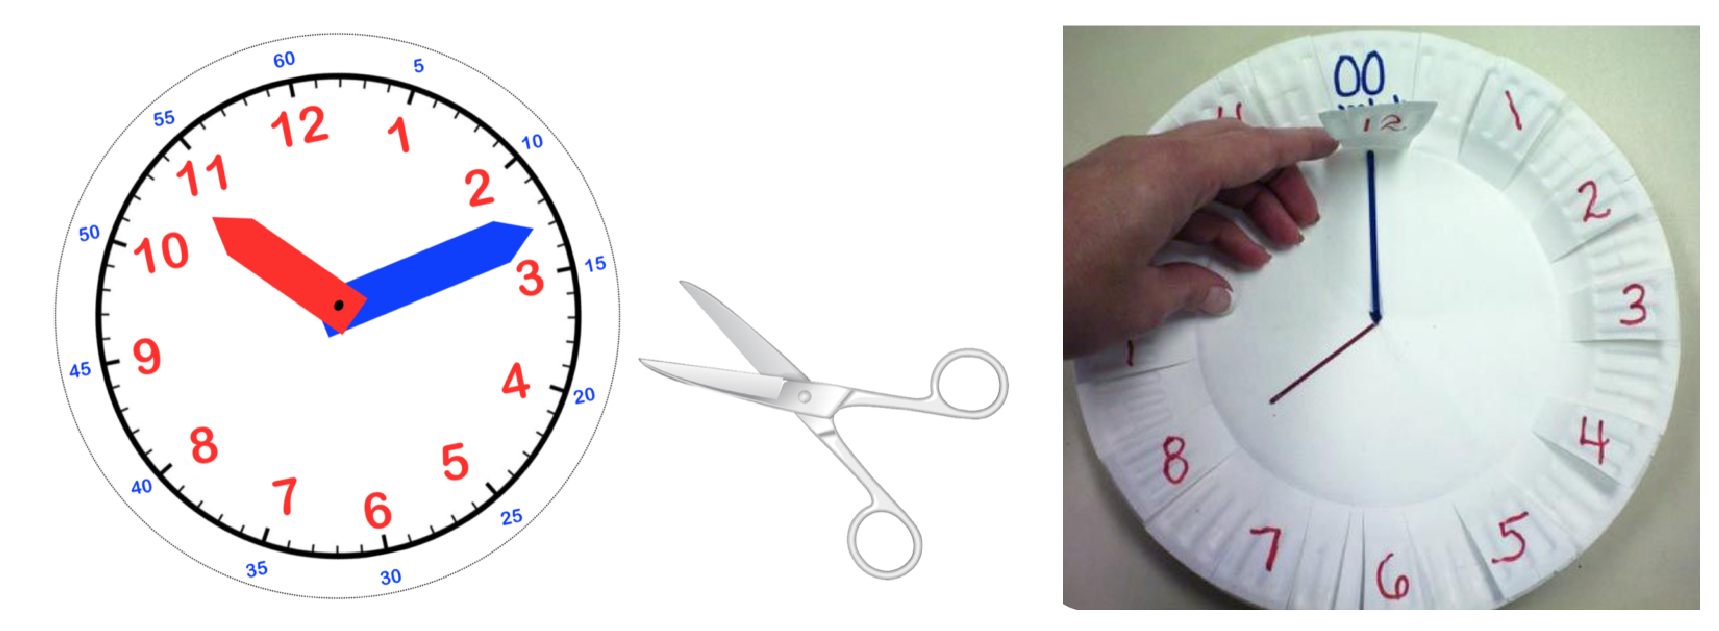
\includegraphics[width=8cm]{Grandeurs_mesures_did/Images/Grm7_cours_horloges} \quad 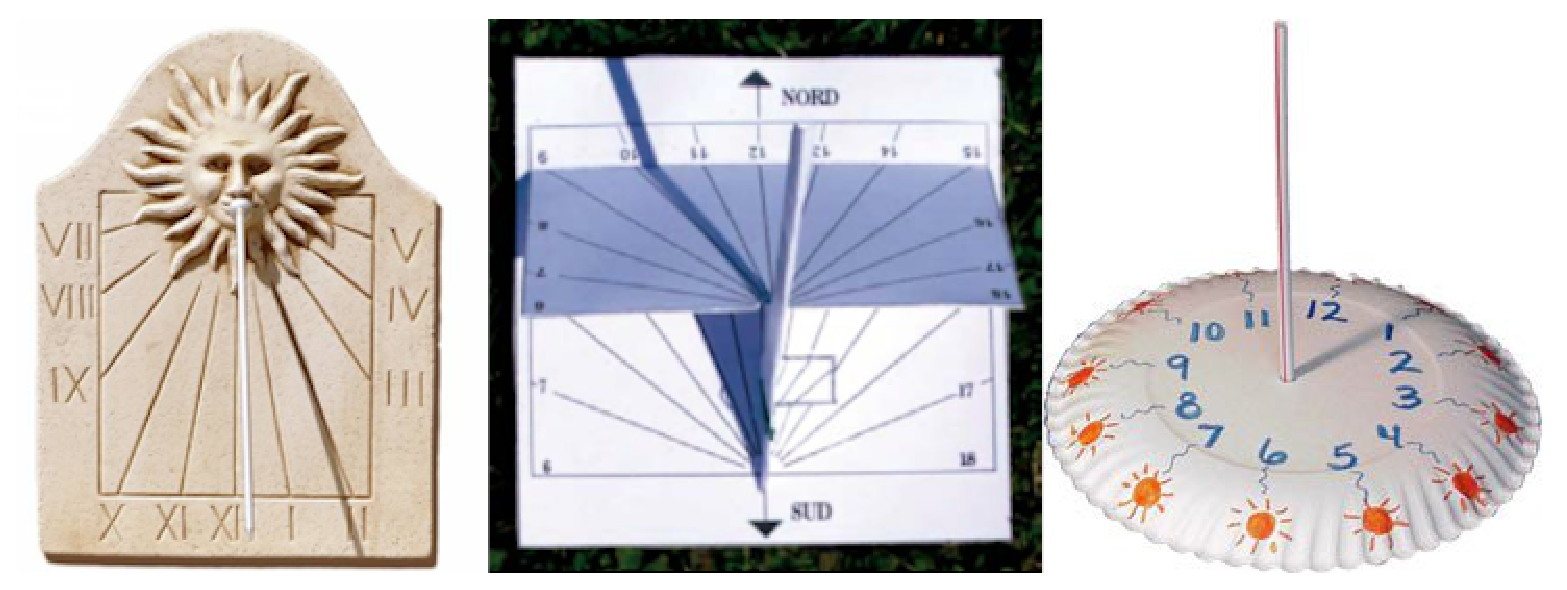
\includegraphics[width=8cm]{Grandeurs_mesures_did/Images/Grm7_cours_cadran_solaire} \\
\end{center}

\pagebreak


\subsection{Le prix} %%%

{\bf -- Au CP}, après un travail préalable sur la construction de la grandeur prix et la notion de valeur, les élèves utilisent l’euro, en manipulant du matériel pièces/billets (pièces de 1 et 2 euros, puis billets de 5 et 10, 20, 50 et 100 euros\dots). \\
{\bf -- Au CE1 et CE2}, les élèves utilisent l’euro et les centimes d’euros dans des situations qui se complexifient progressivement (exemple : rendre la monnaie sur 2 euros pour l’achat d’un produit qui coûte 1 \euro{} 50 c puis 75 c) ; ils résolvent des problèmes impliquant ces données. \\
Il est important de proposer des activités concrètes et connectées avec la réalité des élèves. Ces activités seront centrales, mais pour aller plus loin, on pourra utiliser des tickets de caisse, donner des ordres de grandeur de prix du quotidien, ou encore dessiner les pièces et les billets et analyser les écritures et dessins qui les composent. On pourra également  donner aux élèves des repères historiques sur la monnaie européenne.
\begin{center}
   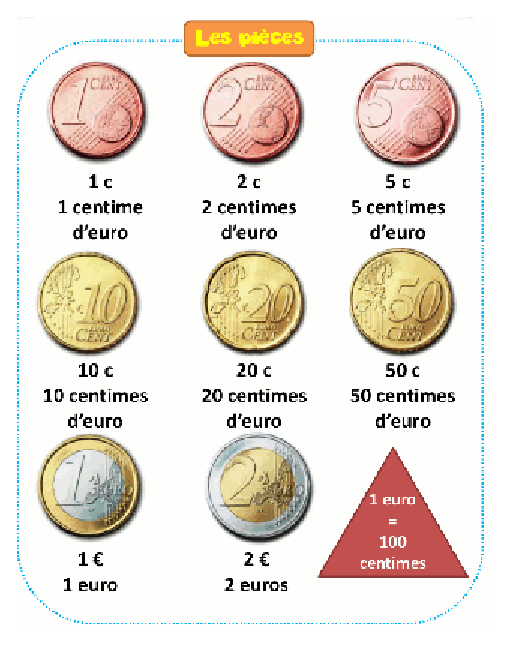
\includegraphics[height=7.5cm]{Grandeurs_mesures_did/Images/Grm7_cours_pieces}
   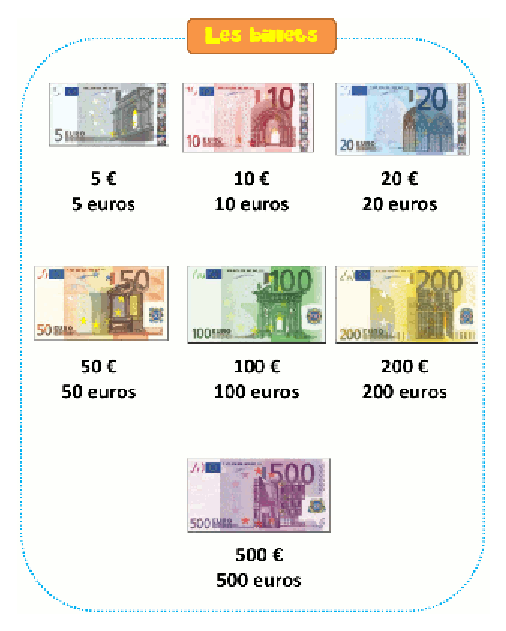
\includegraphics[height=7.5cm]{Grandeurs_mesures_did/Images/Grm7_cours_billets}
\end{center}

Tout comme les autres grandeurs, tout ce qui tourne autour de l'argent à ses propres {\bf expressions} qu'il conviendrait d'expliciter : l'argent ne fait pas le bonheur, avoir le beurre et l'argent du beurre, jeter l'argent par les fenêtres, un sou est un sou\dots \medskip

Une {\bf difficulté} liée à l'euro est qu'il n'existe pas de vocabulaire pour tous les ordres : on trouve en effet l'euro et le centime d'euro (centième d'un euro), mais rien \og entre \fg{} qui pourrait correspondre au dixième d'euro. Ainsi, \og deux euros cinq \fg{} correspondent à 2,05 \euro{}, alors que la plupart du temps, \og deux kilos cinq \fg{} caractérisent \ukg{2,5}, ou encore \ukg{2} et \ug{500}. Le tableau suivant montre les unités qui suivent scrupuleusement le système décimal, et les euros qui dérogent à la règle. Remarquons que le kilo euro (1000 \euro) n'est pas présent au sein du programme de l'école, mais est souvent utilisé dans des domaines économiques. \smallskip

\begin{center}
{\hautab{1.3}
   \begin{CLtableau}{0.8\linewidth}{8}{p{3.5cm}}
      \hline
      Préfixe & kilo & hecto & déca & & déci & centi & milli \\
      \hline
      Unités de longueur & km & hm & dam & m & dm & cm & mm \\
      \hline
      Unités de masse & kg & hg & dag & g & dg & cg & mg \\
      \hline
      Unités de contenance & kL & hL & daL & L & dL & cL & mL \\
      \hline
      Unités de prix & k\euro & & & \euro & & centime d'\euro&  \\
      \hline
   \end{CLtableau}}
\end{center}

 
\subsection{Les aires} %%%

{\bf -- Au CM1}, les élèves comparent des surfaces selon leur aire par estimation visuelle, par superposition ou découpage et recollement. Ils estiment des aires, ou les déterminent, en faisant appel à une aire de référence. Le lien est fait chaque fois que possible avec le travail sur les fractions. \\
{\bf -- Au CM2}, l’utilisation d’une unité de référence est systématique. Cette unité peut être une maille d’un réseau quadrillé adapté, le \ucmq{} , le \udmq{} ou le \umq{}. \\
Les élèves apprennent à utiliser les formules d’aire du carré, du rectangle et du triangle rectangle. \medskip

La mesure des surfaces (aire) est vue au cycle 3. Tout au long du cycle, il convient de choisir la procédure adaptée pour comparer les aires de deux surfaces, pour déterminer la mesure d’une aire avec ou sans recours aux formules.
\begin{center}
   {\small
   \begin{tabular}{p{5cm}p{5cm}p{5cm}}
      \begin{pspicture}(-0.8,-0.5)(3,2.8)
         {\psset{unit=1.3}
         \psframe[fillstyle=solid,fillcolor=A1](0,0)(2.7,2)
         \pcline[offset=10pt]{<->}(0,0)(0,2)\mput*{$\ell$}
         \pcline[offset=-10pt]{<->}(0,0)(2.7,0)\mput*{$L$}
         \rput(1.3,1.2){\white $\mathcal{A}$ = Longueur $\times$ largeur}
         \rput(1.3,0.8){\white $\mathcal{A} = L \times l$}}
      \end{pspicture}
      &
      \begin{pspicture}(-1.2,-0.5)(2,2.8)
         {\psset{unit=1.3}
         \psframe[fillstyle=solid,fillcolor=A2](0,0)(2,2)
         \pcline[offset=10pt]{<->}(0,0)(0,2)\mput*{$c$}
         \pcline[offset=-10pt]{<->}(0,0)(2,0)\mput*{$c$}
         \rput(1,1.2){\white $\mathcal{A}$ = côté $\times$ côté}
         \rput(1,0.8){\white $\mathcal{A}= c \times c = c^2$}}
      \end{pspicture}
      &
      \begin{pspicture}(-1,-0.5)(3,2.8)
         {\psset{unit=1.3}
         \pspolygon[fillstyle=solid,fillcolor=A3](0,0)(2.7,0)(0,2)
         \pcline[offset=10pt]{<->}(0,0)(0,2)\mput*{$h$}
         \pcline[offset=-10pt]{<->}(0,0)(2.7,0)\mput*{$B$}
         \rput(0.9,0.5){\darkgray $\mathcal{A} = \dfrac{B \times h}{2}$}}
      \end{pspicture} \\
      on commencera par des rectangles de dimensions entières, puis de dimensions décimales dont l'une est entière ; enfin, on introduira la formule.
      &
      on commencera par la formule de l'aire du rectangle, puis on présentera celle de l'aire du carré comme un cas particulier de celle du rectangle.
      &
      le triangle rectangle est vu comme un rectangle coupé en deux suivant sa diagonale, la formule peut alors être déduite de celle du rectangle. \\
   \end{tabular}}
\end{center}

Les écritures avec les unités permettent également de renforcer le sens des unités produits. Pour le calcul de l’aire d’un rectangle du type $\ucm{3}\times\ucm{4}$, les élèves proposent souvent le résultat \ucm{12}. \\
On peut justifier l’unité produit par exemple de la façon suivante : \\
$\ucm{3}\times\ucm{4} =(3\times\ucm{1})\times(4\times\ucm{1})$ \\
\hspace*{1.73cm} $= (3\times4)\times(\ucm{1}\times\ucm{1})$ \\
\hspace*{1.73cm} $= 12\times\ucmq{1}$ \\
\hspace*{1.73cm} $= \ucmq{12}$ \\
   Une telle décomposition n’est pas attendue des élèves, mais peut être proposée par l’enseignant, en amont pour renforcer le sens des unités d’aire ou chaque fois que des erreurs d’unité seront constatées chez les élèves. \medskip

Le périmètre et l’aire varient toujours dans le même sens quand on agrandit ou réduit une figure. Ceci n’est plus nécessairement le cas lorsque les figures n’ont plus la même forme : \\
\begin{minipage}{9cm}
    la figure A ci-contre est perçue comme un grand carré amputé d'un petit carré, alors que la figure B est perçue comme un grand carré augmenté d'un petit. Ce qui est exact en terme de décomposition et recomposition. \end{minipage}
\qquad
\begin{minipage}{6.7cm}
   {\psset{unit=0.55}
   \begin{pspicture}(0,-0.3)(12,4.3)
      \pspolygon[fillstyle=solid,fillcolor=B2,linewidth=1.5pt](0,0)(4,0)(4,1)(2,1)(2,3)(4,3)(4,4)(0,4)
      \pspolygon[fillstyle=solid,fillcolor=B2,linewidth=1.5pt](6,0)(10,0)(10,1)(12,1)(12,3)(10,3)(10,4)(10,4)(6,4)
      \psgrid[subgriddiv=1,gridlabels=0,gridcolor=gray](12,4)
      \rput(1,2){\large\bf\white A}
      \rput(8,2){\large\bf\white B}
   \end{pspicture}}
\end{minipage}

Ce qui est erroné, c'est le mouvement de pensée qui traduit cette perception en opération (soustraction ou addition) sur les deux grandeurs périmètre et aire. S'il est vrai qu'à l'addition perceptive des deux formes correspond l'addition des aires, il n’en est pas de même au niveau des périmètres : les deux figures ont en effet le même périmètre. \\
Il est donc nécessaire, après les avoir introduites, de confronter les notions de périmètre et d’aire, afin de permettre aux élèves de bien les différencier, de voir à quoi elles correspondent pour une même figure et de comprendre à travers les exemples rencontrés qu’elles ne sont pas liées. On pourra à cette occasion se nourrir de l'article très complet d'{\it Yves Martin} à propos de \href{http://irem.univ-reunion.fr/spip.php?article802}{Curvica} [mar15]. \medskip

Les {\bf difficultés} suivantes concernant les aires sont assez semblables à celles pour les longueurs, (la surface étant une grandeur produit de deux longueurs) et sont aussi très liées : \\ [1mm]
{\hautab{1.2}
\begin{Ltableau}{\linewidth}{2}{p{5.15cm}|p{10.8cm}}
   \hline
   Compétences & Difficultés ou erreurs \\
   \hline
   Comparer des aires : \newline
   - par superposition \newline
   - par découpage et recollement \newline
   - en utilisant une unité de mesure
   &
   -- L'élève n'est pas conservant des surfaces \newline
   -- L'élève pense que seul le carré peut être une unité acceptable et rencontre des difficultés de manipulation pour paver une figure avec une grandeur unité donnée \newline
   -- L'élève pense que des figures qui ne sont pas directement superposables ne peuvent pas avoir la même aire  \newline
   -- L'élève assimile l'aire à l'encombrement  \\
   \hline
   Estimer la mesure de l'aire d'une surface
   &
   Par manque d'expériences, l'élève n'a aucune idée des mesures de certaines surfaces  \\
   \hline
   Effectuer des conversions d'unité
   &
   L'élève utilise les techniques de conversion qu'il connaît pour les unités de longueur \\
   \hline
\end{Ltableau}}

\medskip

On pourra agir sur les {\bf variables didactiques} suivantes concernant la comparaison d'aires : \\
-- nature des objets dont on demande de comparer les aires : objets physiques ou objets représentés ; \\
-- taille de ces objets ou de la figure ; \\
-- possibilité de superposition directe ou non ; \\
-- présence de quadrillage ou non ; \\
-- possibilité ou non de décomposer un objet pour tenter de reconstituer un objet superposable à un autre.

\bigskip


\subsection{Les angles} %%%

\smallskip

{\bf -- Au CE1 et CE2}, les élèves utilisent l’équerre pour tracer ou reconnaître des angles droits. \\
{\bf -- Au CM1 et CM2}, les élèves apprennent à repérer les angles d’une figure plane, puis à comparer ces angles par superposition (utilisation du papier calque) ou en utilisant un gabarit. Ils estiment, puis vérifient en utilisant l’équerre, qu’un angle est droit, aigu ou obtus. \\
{\bf -- Au collège}, ce travail sera poursuivi et l’on introduira une unité de mesure des angles (le degré) et l’utilisation d’un outil de mesure (le rapporteur). \medskip

La mesure n'étant pas du ressort de l'école primaire, on aura uniquement recours à des comparaisons d'angles par superposition, avec un calque ou un gabarit. Seul l'angle droit pourra être déduit grâce à l'équerre ou le gabarit d'angle droit. \\
L'angle droit est introduit au cycle 2, et au cycle 3, la notion d’angle peut être abordée comme \og l’ouverture \fg{} définie par deux demi-droites de même origine. Les élèves doivent comprendre que l’angle ne change pas lorsque l’on prolonge ces demi-droites.
\begin{center}
   \begin{pspicture}(-0.5,0)(9,3)
      \psline(2;15)(0;0)(2;75)
      \rput(3;0){\psline[linestyle=dashed](5;0)(0,0)(5;30)}
      \psset{linewidth=1.5pt}
      \psarc[linecolor=A1](0,0){.5}{15}{75}
      \psarc[linecolor=A1](0,0){.6}{15}{75}
      \psarc[linecolor=B2](3,0){.8}{0}{30}
      \rput(9,1.25){$\Longrightarrow$}
   \end{pspicture}
   \begin{pspicture}(-1,0)(6,3.5)
      \psline[linestyle=dashed](5;15)(0,0)(5;45)
     \psline(2;15)(0;0)(2;75)
      \psset{linewidth=1.5pt}
      \psarc[linecolor=A1](0,0){.5}{15}{75}
      \psarc[linecolor=A1](0,0){.6}{15}{75}
      \psarc[linecolor=B2](0,0){.8}{15}{45}
      \rput(2.5,-0.5){\small L'angle bleu est plus grand que l'angle rouge}
   \end{pspicture}
\end{center}


%%%%%%%%
\activites %%%
%%%%%%%%

\textcolor{G1}{Sujet proposé aux M2 par la FDE de Montpellier, 2022} \\

{\bf\uline{Consigne}} : Vous êtes enseignant(e) en classe de MS. Vous avez déjà mené avec vos élèves l’activité décrite dans le document 1. \\
Vous construirez une séance qui fait suite à cette activité et permet de travailler la compétence visée. Vous pourrez notamment vous inspirer des images proposées en annexes 2 et 3. \\

{\bf\uline{Compétence visée}} : Classer ou ranger des objets selon un critère de longueur ou de masse ou de contenance. \\

{\bf\uline{Contexte de la séance d'enseignement}} : \\
   \hspace*{5mm} -- cycle d'enseignement : cycle 1 ; \\
   \hspace*{5mm} -- niveau de la classe : MS ; \\
   \hspace*{5mm} -- domaine : Explorer des formes, des grandeurs, des suites organisées ; \\ [3mm]
  

{\bf\uline{Documents fournis au candidat}} : \\

{\bf\uline{Document 1}} : Extrait du programme consolidé de cycle 1 publié au BO n°25 du 24/06/2021. \medskip

\begin{center}
   \begin{minipage}{15cm}
      \textsf{{\textcolor{teal}{\bf 4.2. Explorer des formes, des grandeurs, des suites organisées}} \\ [1mm]
      Très tôt, les jeunes enfants discernent intuitivement des formes (carré, triangle, etc.) et des grandeurs (longueur, contenance, masse, aire, etc.). À l’école maternelle, ils construisent des connaissances et des repères sur quelques formes et grandeurs. L’approche des formes planes, des objets de l’espace, des grandeurs, se fait par la perception visuelle, la manipulation et la coordination d’actions sur des objets. Cette approche est soutenue par le langage : il permet de décrire ces objets et ces actions et favorise l’identification de premières caractéristiques descriptives. Ces connaissances qui resteront limitées constituent une première approche de la géométrie et de la mesure qui seront enseignées aux cycles 2 et 3. \\ [3mm]
      {\bf\textcolor{teal}{4.2.1. Objectifs visés et éléments de progressivité}} \\ [1mm]
      Très tôt, les enfants regroupent les objets, soit en fonction de leur aspect, soit en fonction de leur utilisation familière ou de leurs effets. À l’école, ils sont incités à « mettre ensemble ce qui va ensemble » pour comprendre que tout objet peut appartenir à plusieurs catégories et que certains objets ne peuvent pas appartenir à celles-ci. \\
      Par des observations, des comparaisons, des tris, les enfants sont amenés à mieux distinguer différents types de critères : forme, longueur, masse, contenance essentiellement. Ils apprennent progressivement à reconnaître, distinguer, décrire des solides puis des formes planes. Ils commencent à appréhender la notion d’alignement qu’ils peuvent aussi expérimenter dans les séances d’activités physiques. L’enseignant est attentif au fait que l’appréhension des formes planes est plus abstraite que celle des solides et que certains termes prêtent à confusion (carré/cube). L’enseignant utilise un vocabulaire précis (cube, boule, pyramide, cylindre, carré, rectangle, triangle, cercle ou disque - à préférer à \og rond \fg) que les enfants sont entraînés ainsi à comprendre d’abord puis amenés progressivement à utiliser. \\
      Par ailleurs, dès la petite section, les enfants sont invités à organiser des suites d’objets en fonction de critères de formes et de couleurs ; les premiers algorithmes qui leur sont proposés sont constitués d’alternances simples. Dans les années suivantes, progressivement, ils sont amenés à reconnaître un rythme dans une suite organisée et à continuer cette suite, à inventer des \og rythmes \fg{} de plus en plus compliqués, à compléter des manques dans une suite organisée.}
   \end{minipage}
\end{center}

\pagebreak


{\bf\uline{Document 2}} : Extrait de {\it Découvrir les maths}, MS. Dominique Valentin, 2015. pp. 61 et 62. 

\begin{center}
   \fbox{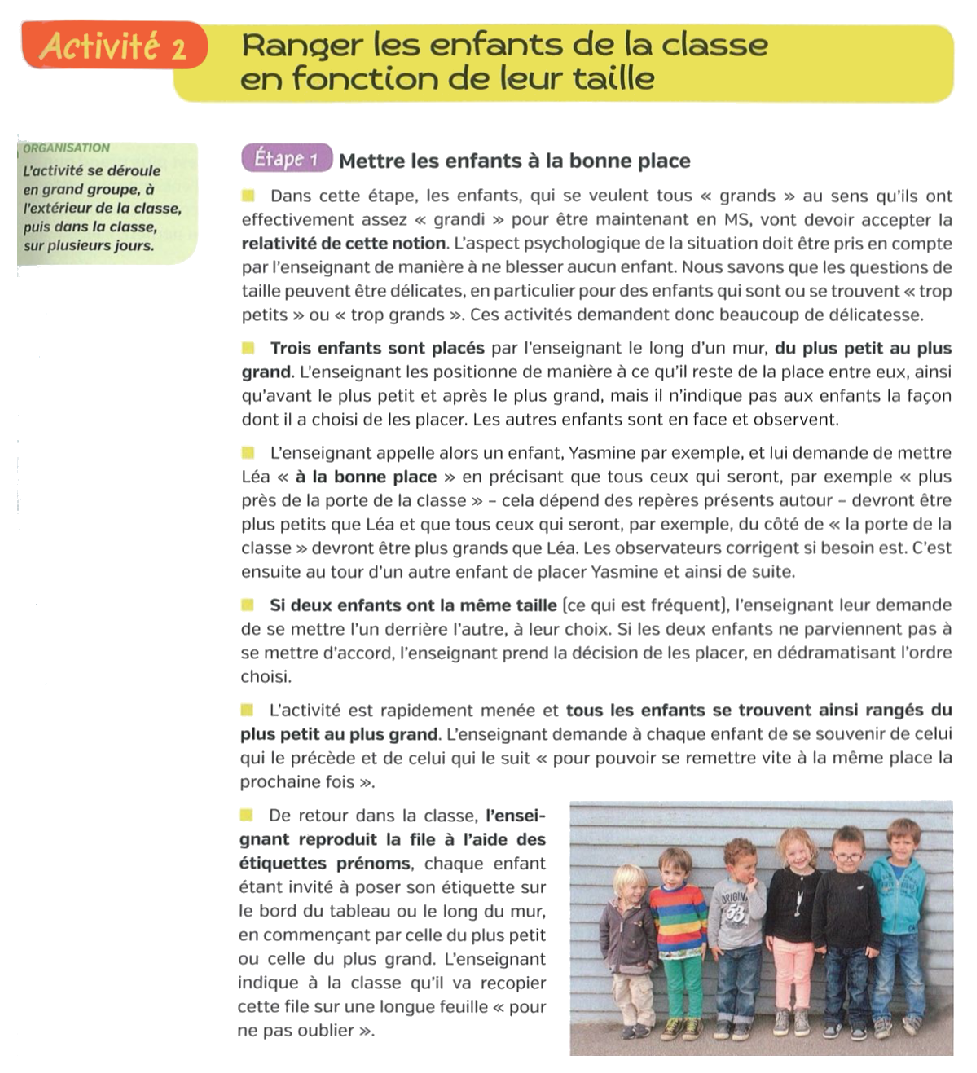
\includegraphics[width=16.5cm]{Grandeurs_mesures_did/Images/Grm7_crpe_taille1}} \\ [3cm]
\end{center}

\pagebreak


\begin{center}
   \fbox{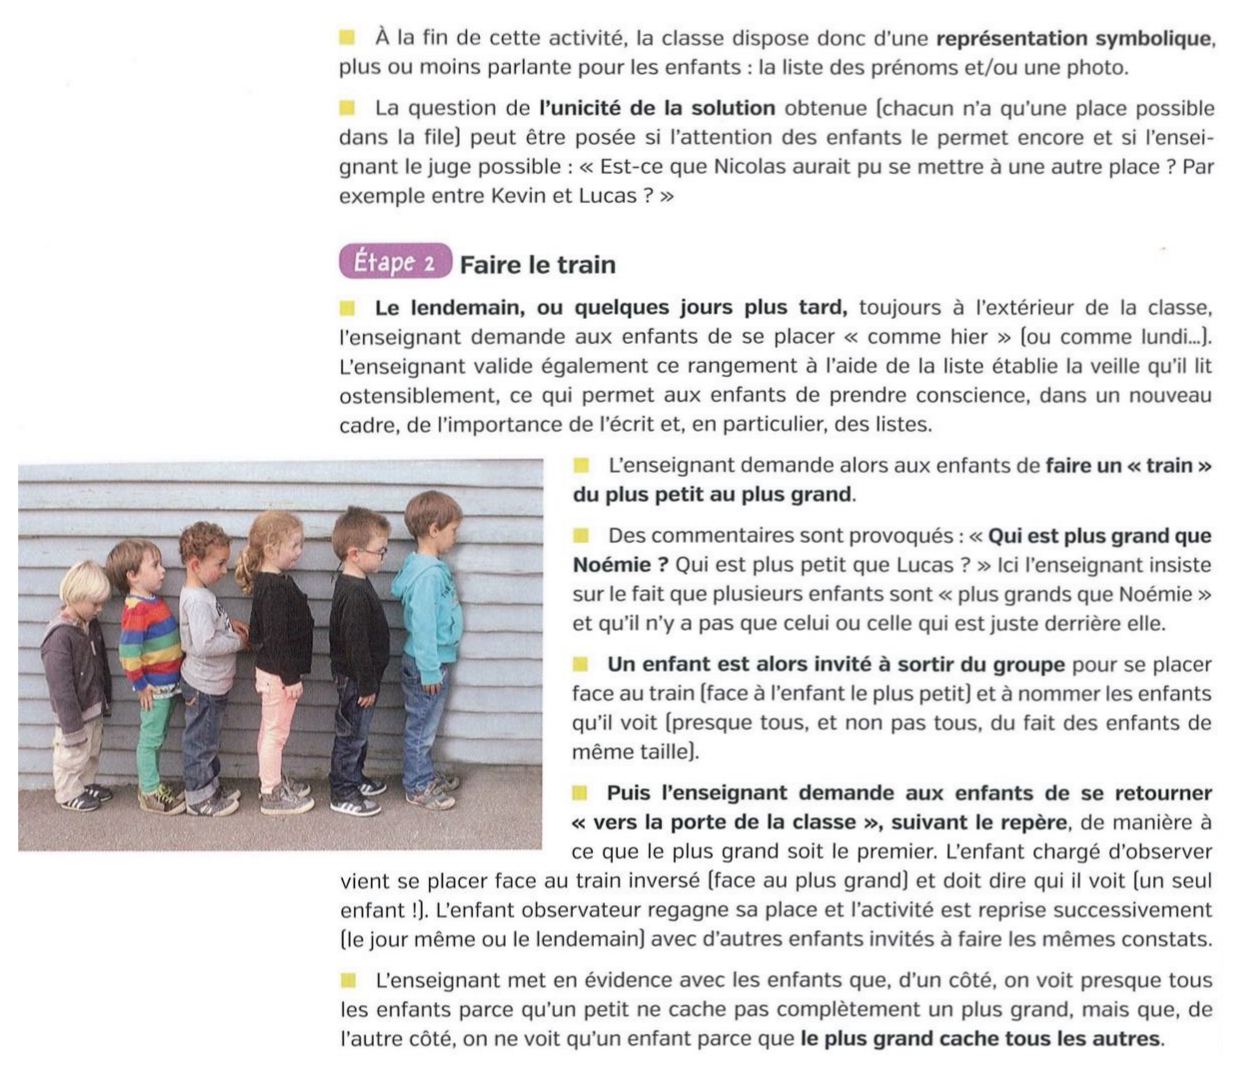
\includegraphics[width=16.5cm]{Grandeurs_mesures_did/Images/Grm7_crpe_taille2}}
\end{center}

\ \\


\begin{minipage}{8cm}
   {\bf\uline{Document 2}} : Image issue de {\it vers les maths}, GS. Accès 2011. p. 59. \\ [2mm]
   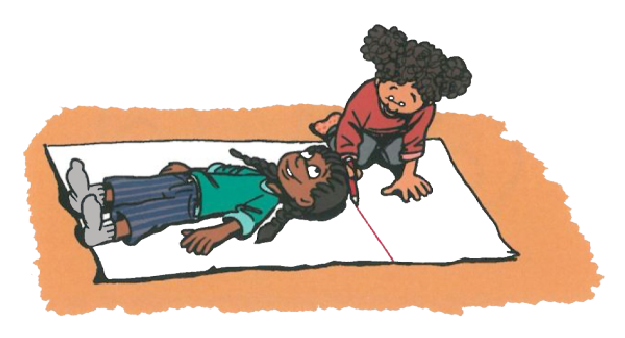
\includegraphics[width=8cm]{Grandeurs_mesures_did/Images/Grm7_crpe_taille3}
\end{minipage}
\qquad
\begin{minipage}{8cm}
   {\bf\uline{Document 3}} : Image issue du site de l'Académie de Nancy-Metz. \\ [2mm] 
   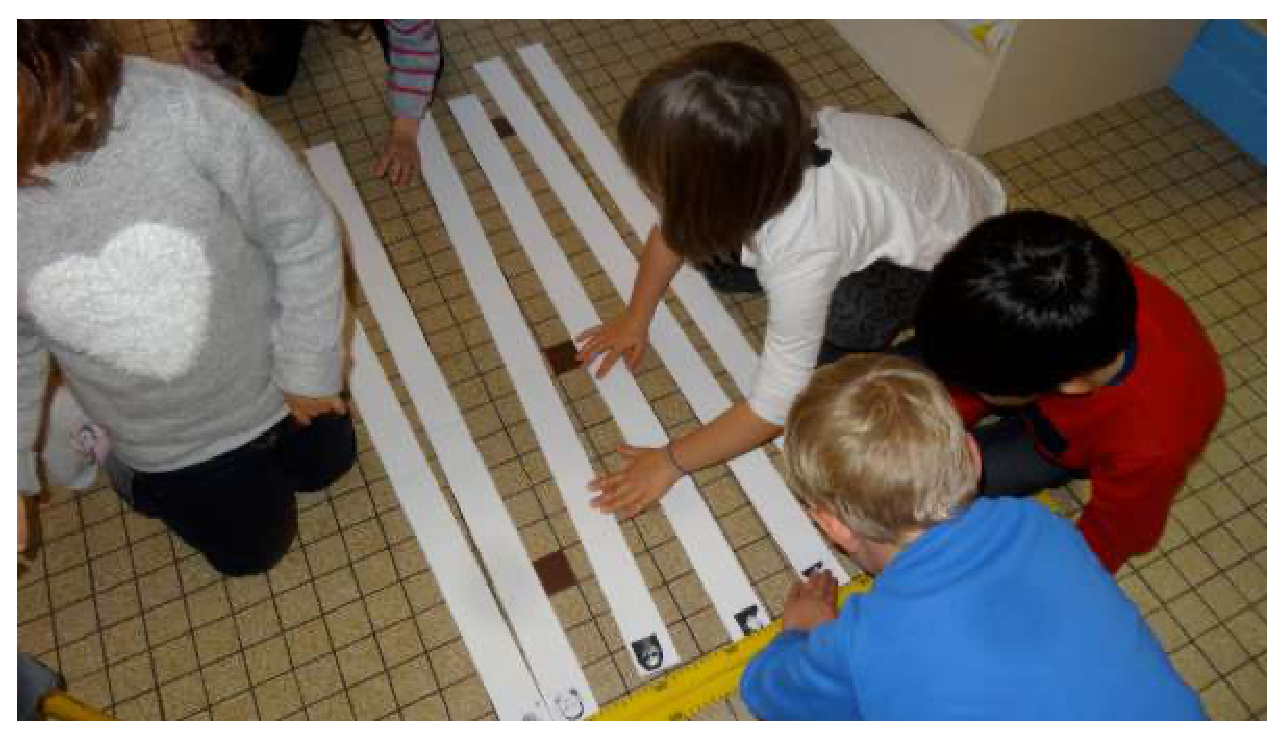
\includegraphics[width=8cm]{Grandeurs_mesures_did/Images/Grm7_crpe_taille4}
\end{minipage}



%%%%%%%%
\analyses %%%
%%%%%%%%

%%%%%%%%%%%%%%%%%%%%%%%%%%%%%%%
%\begin{exercice*}[CRPE 2006 G3]
%Observer les trois problèmes présentés ci-dessous. Ils sont extrait d'un manuel de la collection {\it Cap maths}, éditions Hatier, 2004.
%\begin{enumerate}
%   \item Dans quel cycle de l'école primaire ces problèmes pourraient-ils être traités ? Justifier la réponse.
%   \item Proposer deux erreurs de procédure que pourraient commettre des élèves dans le problème 1.
%   \item Indiquer les principales étapes de la procédure que pourrait adopter un élève pour résoudre le problème 2.
%   \item Quelles connaissances supplémentaires par rapport aux deux problèmes précédents, la résolution du problème 3 suppose-t-elle ? \\
%\end{enumerate}
%
%\begin{center}
%\fbox{
%\begin{minipage}{15cm}   
%{\large\bf Quelles sont les mesures des étiquettes ?} \\
%   \begin{minipage}{7cm}
%      (1) Les étiquettes rouges qui constituent ce rectangle sont toutes identiques. Le dessin n'est pas en vraie grandeur. Trouve la longueur et la largeur de chaque étiquette.
%   \end{minipage}
%   \qquad
%   \begin{minipage}{7cm}
%      {\psset{unit=0.4}
%      \begin{pspicture}(-1,-1)(13,12)
%         \psframe[fillstyle=solid,fillcolor=B2](0,0)(12,10)
%         \psline(4,0)(4,6)
%         \psline(8,0)(8,6)
%         \psline(6,6)(6,10)
%         \psline(0,6)(12,6)
%         \pcline[offset=-3mm]{<->}(12,0)(12,10)
%         \lput*{:U}{10 cm}
%         \pcline[offset=3mm]{<->}(0,10)(12,10)
%         \lput*{:U}{12 cm}
%      \end{pspicture}}
%   \end{minipage}
%   
%   \begin{minipage}{7cm}
%      (2) Les étiquettes bleues déjà placées sur ce rectangle sont toutes identiques. Le dessin n'est pas en vraie grandeur. Trouve la longueur et la largeur de chaque étiquette.
%   \end{minipage}
%   \qquad
%   \begin{minipage}{7cm}
%      {\psset{unit=0.3}
%      \begin{pspicture}(-1,-1)(19,18)
%         \pspolygon[fillstyle=solid,fillcolor=A1](12,0)(18,0)(18,16)(0,16)(0,14)(16,14)(16,2)(12,2)
%         \psline(0,14)(0,0)(14,0)
%         \psline(16,2)(18,2)
%         \psline(16,8)(18,8)
%         \psline(16,14)(18,14)
%         \psline(6,14)(6,16)
%         \psline(12,14)(12,16)
%         \pcline[offset=-3mm]{<->}(18,0)(18,16)
%         \lput*{:U}{16 cm}
%         \pcline[offset=3mm]{<->}(0,16)(18,16)
%         \lput*{:U}{18 cm}
%      \end{pspicture}}
%   \end{minipage}
%
%   \begin{minipage}{7cm}
%      (3) Ces étiquettes vertes, toutes identiques, sont disposées à l'intérieur d'un carré. Le périmètre de ce carré mesure 96 cm. Le dessin n'est pas en vraie grandeur.
%      \begin{enumerate}
%         \item[a.] Trouve la longueur et la largeur de chaque étiquette.
%         \item[b.] Trouve le périmètre du carré blanc.
%      \end{enumerate}
%   \end{minipage}
%   \qquad
%   \begin{minipage}{7cm}
%      {\psset{unit=0.2}
%      \begin{pspicture}(-2,-2)(25,26)
%         \psframe[fillstyle=solid,fillcolor=G1](0,0)(24,24)
%         \psline(0,4)(24,4)      
%         \psline(0,12)(24,12)
%         \psline(0,20)(24,20)
%         \psline(8,0)(8,24)
%         \psline(16,0)(16,24)
%         \psframe[fillstyle=solid,fillcolor=white](4,4)(20,20)
%      \end{pspicture}}
%   \end{minipage}
%\end{minipage}}
%\end{center}
%\end{exercice*}
%
%\begin{corrige}
%\ \\ [-5mm]
%\begin{enumerate}
%   \item La notion de périmètre d'un rectangle et la formule du périmètre du carré/rectangle apparaissent au C3. \\
%   \item Les erreurs possibles :
%   \begin{itemize}
%      \item l'élève mesure les côtés sur le dessin et ne tient pas compte du fait que le dessin n'est pas en vraie grandeur ;
%      \item l'élève divise les dimensions du grand rectangle par 5 car il y a 5 rectangles identique pour paver le grand et fournit donc le résultat \og longueur de 2,4 cm et largeur de 2 cm \fg.
%   \end{itemize}
%   \item Les étapes possibles : \\
%   \begin{itemize}
%      \item la longueur du grand rectangle, 18 cm correspond à 3 fois celle de l'étiquette. La longueur de l'étiquette est donc 6 cm ($\ucm{18}\div3 =\ucm{6}$) ;
%      \item la largeur du grand rectangle, 16 cm correspond à 2 fois la longueur ($2\times\ucm{6} =\ucm{12}$) de l'étiquette augmentée de 2 fois la largeur de l'étiquette. Par différence, 2 fois la largeur de l'étiquette mesure \\
%      16 cm $-$ 12 cm = 4 cm. La largeur de l'étiquette est donc 2 cm ($\ucm{4}\div2$).
%   \end{itemize}
%   \item Ce problème fait appel à la compétence \og calculer le périmètre d'un carré \fg. Cette notion doit être utilisée dans les deux sens : à partir du périmètre, déduire le côté et à partir du côté, déduire le périmètre.
%\end{enumerate}
%\end{corrige}
%%%%%%%%%%%%%%%%%%%%%%%%%%%%%%
%
%\bigskip

%%%%%%%%%%%%%%%%%%%%%%%%%%%%%%
\begin{exercice}[CRPE 2009 G4]
Le document ci-dessous est tiré de \og J'apprends les maths - CE2 \fg, Editions Retz, Séquence 103, page 150.
\begin{center}
   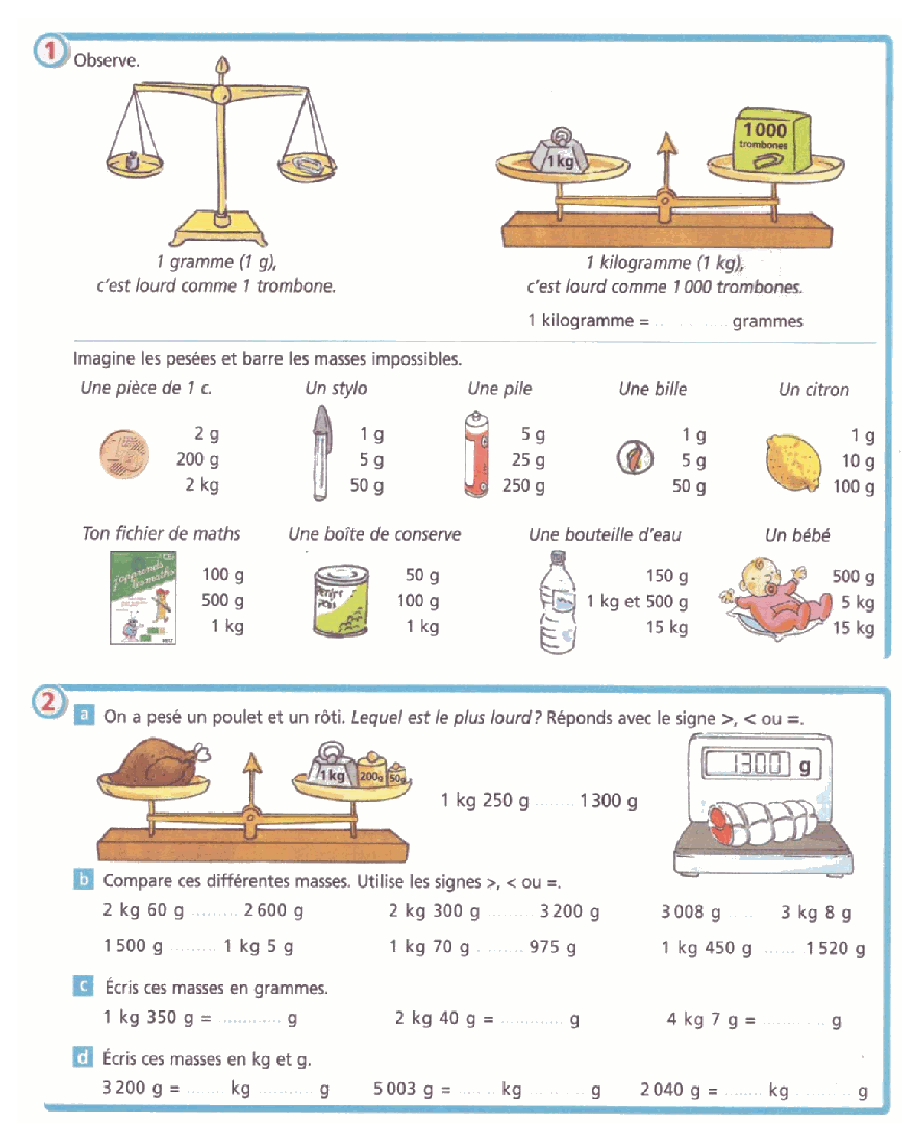
\includegraphics[width=15cm]{Grandeurs_mesures_did/Images/Grm7_analyse_masse_sujet}
\end{center}
\begin{enumerate}
   \item 
   \begin{enumerate}
      \item Citer deux difficultés que peuvent rencontrer les élèves pour barrer les masses impossibles de l'exercice 1.
      \item Citer deux difficultés que peuvent rencontrer les élèves pour répondre correctement à l'exercice 2-a.
   \end{enumerate}
   \pagebreak
   \item Pour cette question, on se reporte à la production d'élève suivante :
   \begin{center}
   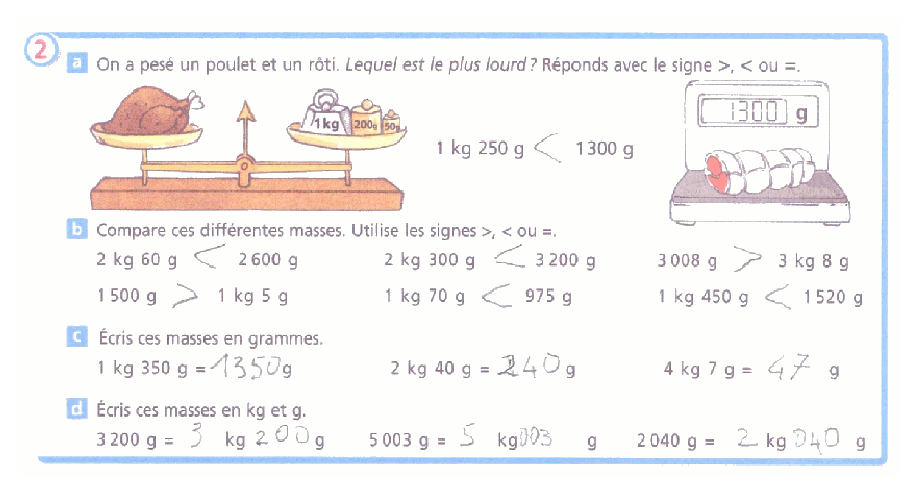
\includegraphics[width=15cm]{Grandeurs_mesures_did/Images/Grm7_analyse_masse_eleve}
   \end{center}
   \begin{enumerate}
      \item Dans cette question on s'intéresse aux exercices 2-a, 2-b et 2-c. Quelle est la règle implicite utilisée par cet élève ?
      \item Dans cette question on s'intéresse à l'exercice 2-d. Lorsqu'il s'agit de transformer une écriture en gramme en une écriture complexe kilogramme-gramme, on peut supposer que l'élève utilise la règle implicite suivante : le premier chiffre correspond au nombre de kilogrammes, le reste des chiffres correspond au nombre de grammes. Proposer un exercice (dans le même contexte) qui permettrait de vérifier si l'élève utilise cette règle qui donne en général un résultat faux.
   \end{enumerate}
   \ \\ [-15mm]
   \item Pour cette question, on se reporte de nouveau à la production d'élève.
   \begin{enumerate}
      \item Comment utiliser des masses marquées et une balance à affichage digital pour faire prendre conscience à l'élève de son erreur lors de l'écriture de l'égalité : 2 kg 40 g = 240 g ?
      \item Donner une aide possible que l'enseignant peut apporter à cet élève.
   \end{enumerate}
\end{enumerate}
\end{exercice}

\begin{corrige}
\ \\ [-5mm]
\begin{enumerate}
   \item 
   \begin{enumerate}
      \item Difficultés de l'exercice 1 :
      \begin{itemize}
         \item les élèves peuvent ne pas bien estimer la masse des objets parce qu'ils ne les ont jamais soupesés ;
         \item l'élève peut avoir du mal à imaginer les masses autre que 1 g ou 1 kg indiquées au début de l'exercice ;
         \item certains objets proposent des masses avec des unités différentes (grammes et kilogrammes).
      \end{itemize}
      \item Difficultés de l'exercice 2-a :
      \begin{itemize}
         \item difficulté dans la conversion des unités (1 kg 250 g correspondent à 1 250 g ou inversement) ;
         \item méconnaissance des signes > et < ;
         \item représentations des masses à l'aide de deux objets différents (balance électronique et balance de Roberval).
      \end{itemize}
   \end{enumerate}
   \setcounter{enumi}{1}
   \item   
   \begin{enumerate}
      \item L'élève n'apporte aucune importance à l'unité et au fait que 1 kg représente 1 000 g : il associe entre eux les différents nombres représentant les masses. Par exemple, 2 kg 300 g = 2 300 g.
      \item Si on a un nombre non composé de 4 chiffres, ce procédé ne fonctionne pas. \\
      Par exemple, 23 456 g donnerait 2 kg et 3 456 g et 123 g ferait 1 kg et 23 g.
   \end{enumerate}
   \setcounter{enumi}{2}
   \item 
   \begin{enumerate}
      \item On peut utiliser deux masses marquées de 1 kg et quatre masses de 10 g et les poser sur la balance digitale, pour que l'élève s'aperçoive qu'en fait, la masse totale est de 2 040 grammes et non pas 240 grammes.
      \item L'enseignant peut par exemple reprendre avec l'élève les masses marquées et lui faire tenir dans une main une masse de 1 g, et dans l'autre celle de 1 kg afin qu'il s'aperçoive de la grande différence de poids, puis effectuer avec lui des conversions toujours en utilisant la manipulation de masses marquées.
   \end{enumerate}
\end{enumerate}
\end{corrige}

\bigskip

\begin{exercice}[CRPE 2016 G2]
   Dans une classe de CM2, un professeur propose le travail suivant aux élèves.
   \begin{center}
   \fbox{
   \begin{pspicture}(0,0)(7,0)
      \rput(3.8,4){Quelle est l'aire, en \ucmq{}, de la figure grisée ?}
      \psframe[fillstyle=solid,fillcolor=lightgray](3,2)(4,3)
      \psline(3,2)(4,3)
      \psline(3,3)(4,2)
      \rput(3,1){4 triangles = \ucmq{1}}
   \end{pspicture}
   \qquad
   \begin{pspicture*}(5,0)(10,5)
      \pspolygon[fillstyle=solid,fillcolor=lightgray](6,0)(9,0)(9,1)(10,2)(8,4)(9,4)(8,5)(7,5)(6,4)(7,4)(5,2)(6,1)
      \pspolygon[fillstyle=solid,fillcolor=white](6.5,0.5)(7.5,1.5)(8.5,0.5)(9,1)(9,2)(8,2)(7.5,2.5)(8,3)(7.5,3.5)(8,4)(7,4)(7.5,3.5)(7,3)(7.5,2.5)(7,2)(6,2)(6,1)
      \psgrid[subgriddiv=1](5,0)(10,5)
      \multido{\i=10+-1}{10}{%
	\FPeval{a}{\i+5}
	\psline(\i,0)(\a,5)
	\psline(\i,5)(\a,0)
	}
   \end{pspicture*}
   }
   \end{center}
   Les productions de quatre élèves sont présentées page suivante.
   \begin{enumerate}
      \item Pour les productions de Raphaëlle et Terry, citer trois compétences qui semblent acquises et analyser les éventuelles erreurs.
      \item Pour les productions de Clément et Cloé, analyser les procédures en pointant les éléments qui les rapprochent et ceux qui les séparent.
   \end{enumerate}
   \begin{center}
      Production de Raphaëlle \\ [2mm]
      \fbox{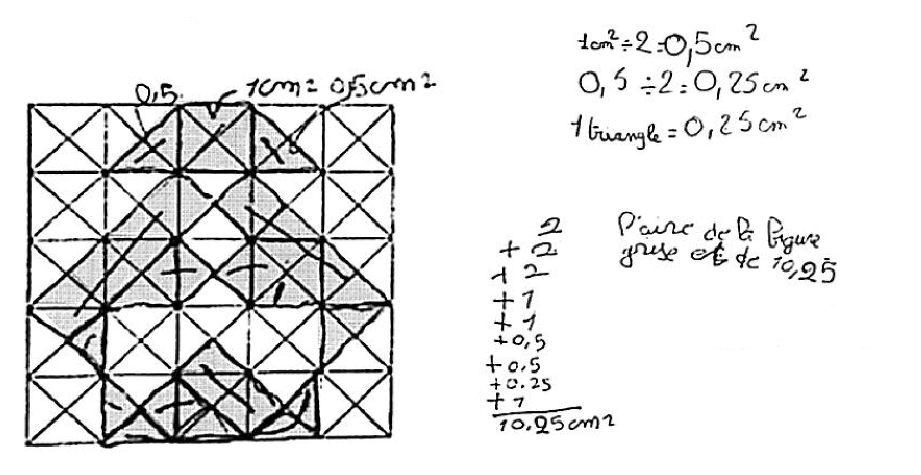
\includegraphics[width=14cm]{Grandeurs_mesures_did/Images/Grm7_analyse_Raphaelle}} \\ [2mm]   
      Production de Terry \hspace{3cm} Production de Clément \\ [2mm] 
      \fbox{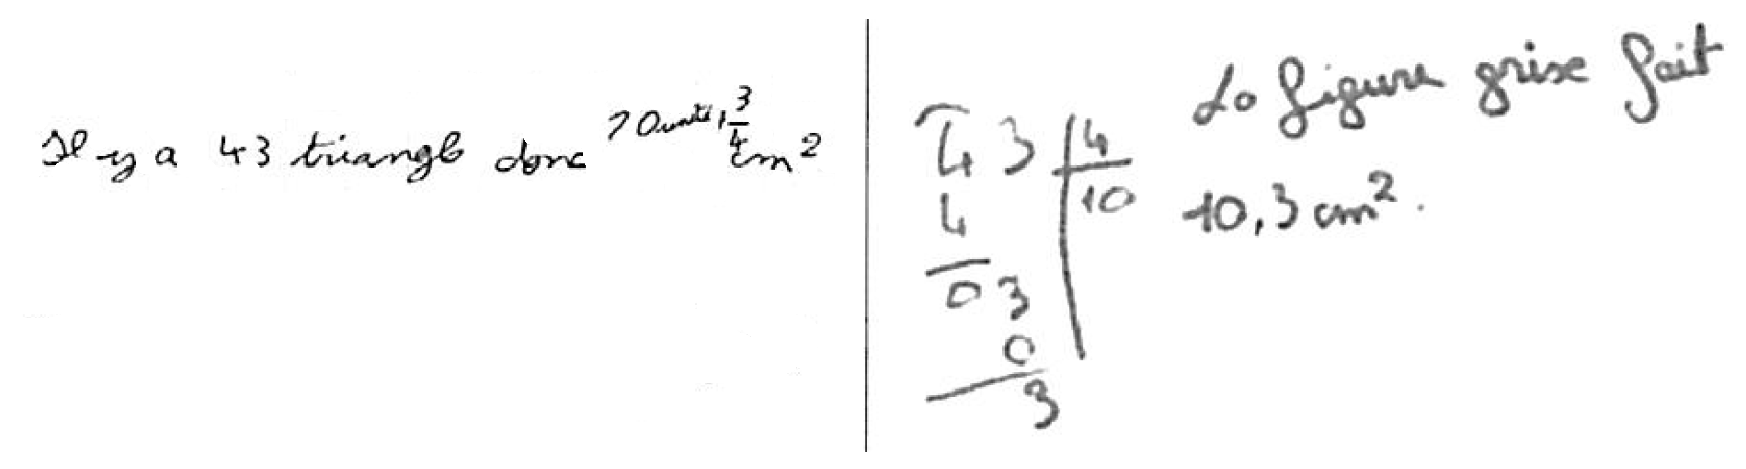
\includegraphics[width=14cm]{Grandeurs_mesures_did/Images/Grm7_analyse_Terry_Clement}} \\ [2mm] 
      Production de Chloé \\ [2mm]
      \fbox{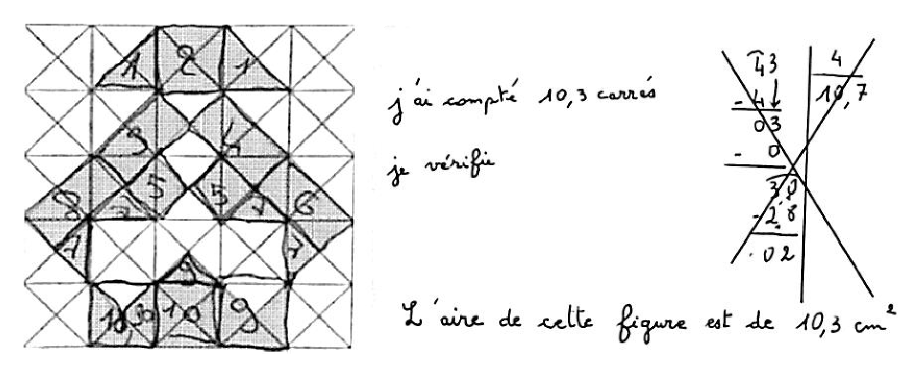
\includegraphics[width=14cm]{Grandeurs_mesures_did/Images/Grm7_analyse_Chloe}}
   \end{center} 
\end{exercice}

\begin{corrige}
\ \\ [-5mm]
\begin{enumerate}
   \item {\bf Compétences} acquises par Raphaëlle  et de Terry :
   \begin{itemize}
      \item ajouter des grandeurs, en particulier des aires : ils savent déterminer une aire complexe par ajout d'aires de figures plus simples ;
      \item mesurer des grandeurs, en particulier des aires : ils savent déterminer l'aire d'un triangle rectangle, à partir de l'aire d'un carré ;
      \item manipuler des nombres décimaux (pour Raphaëlle) : en particulier, calcul de la moitié et du quart d'un entier, addition de nombres décimaux ; et des fractions (pour Terry) : transformation de 43 triangles valant un quart de \ucmq{} en \ucmq{10} plus trois quarts de \ucmq{}.
   \end{itemize}
   {\bf Erreurs} commises par Raphaëlle et Terry :
   \begin{itemize}
      \item le raisonnement de Raphaëlle est correct, mais elle fait une erreur de dénombrement des petits triangles (il lui manque un demi carré). De plus, certaines unités sont manquantes, en particulier dans la réponse ;
      \item la réponse de Terry est juste mais manque d'éléments de rédaction.
   \end{itemize}
   \item \textcolor{A1}{$\bullet$} Les deux élèves comptent correctement des petits triangles et ont conscience qu'il faut diviser ce nombre par 4 pour obtenir l'aire de la figure, ils semblent avoir acquis la compétence \og mesurer une aire \fg ;
   \begin{itemize}
      \item les deux élèves entreprennent une division mais ne vont pas suffisamment loin dans sa résolution : Clément effectue une division euclidienne mais fait une erreur d'interprétations du résultat obtenu : le quotient est 10, le reste 3, ce qu'il écrit 10,3. Il manque a Cloé une dernière étape afin de trouver le résultat exact de 10,75, certainement parce que son résultat intermédiaire (10,7) ne correspond pas à la valeur trouvée de 10,3 ;
      \item Clément utilise la division comme outil pour trouver la réponse alors que Cloé utilise la division comme élément de vérification, elle a dénombré 10 carrés entiers et 3 petits triangles qu'elle interprète comme $10 + 0,3$ ;
      \item le résultat trouvé est le même pour Clément et Cloé (mais il est faux).
   \end{itemize}
\end{enumerate}
\end{corrige}

\bigskip


\begin{exercice}[CRPE 2016 G3]
\begin{minipage}{12cm}
   Un maître a distribué à ses élèves de CM1 des gabarits de lettres et leur a demandé de trouver la longueur de leur contour. Un groupe de trois élèves est chargé de travailler sur le gabarit de la lettre C.
\end{minipage}
\qquad
\begin{minipage}{4cm}
      
\includegraphics[width=3cm]{Grandeurs_mesures_did/Images/Grm7_analyse_TC}
\end{minipage}
\begin{enumerate}
   \item Donner quatre compétences nécessaires pour déterminer la longueur du contour.
   \item Donner deux difficultés que les élèves pourraient rencontrer pour cette tâche.
   \item Voici ci-dessous les productions de trois élèves (Corantin, César et Clarisse). Pour chacun de ces travaux :
   \begin{enumerate}
      \item Analyser la trace écrite (procédures suivies, compétences mises en oeuvre, erreurs éventuelles).
      \item Proposer une remédiation que le professeur pourrait mettre en place pour César et Corantin.
   \end{enumerate}
\end{enumerate}
\begin{center}
   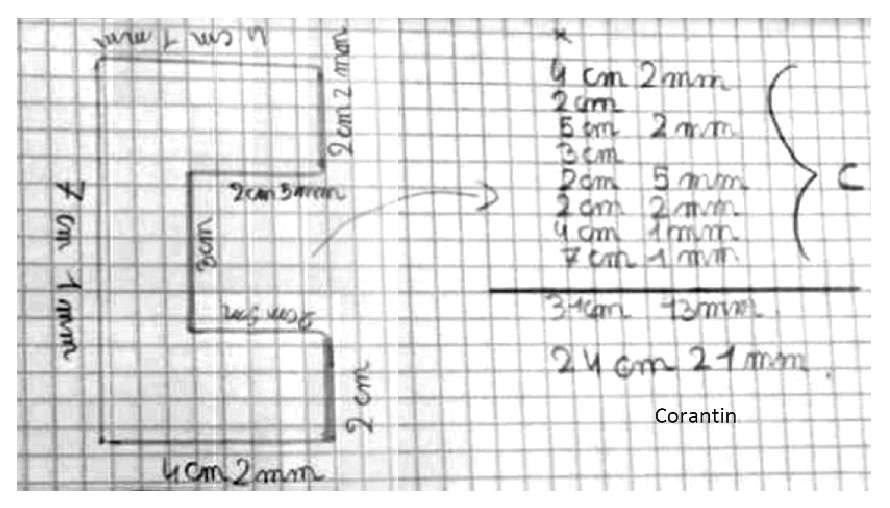
\includegraphics[height=7.5cm]{Grandeurs_mesures_did/Images/Grm7_analyse_TC_Corantin} \\ [5mm]
   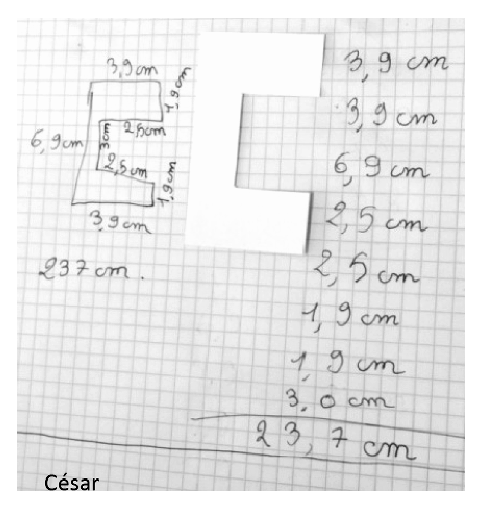
\includegraphics[height=7.5cm]{Grandeurs_mesures_did/Images/Grm7_analyse_TC_Cesar}
   \quad
   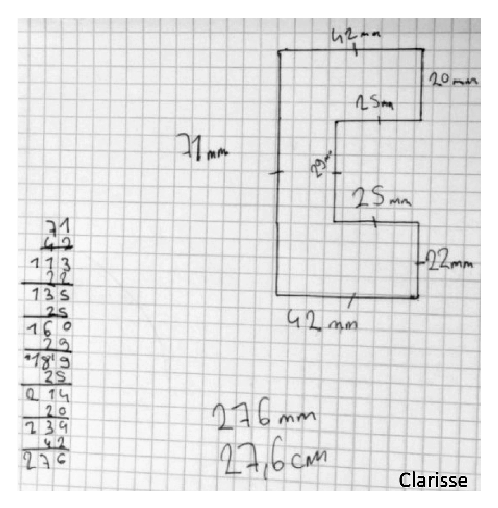
\includegraphics[height=7.5cm]{Grandeurs_mesures_did/Images/Grm7_analyse_TC_Clarisse}
\end{center}
\end{exercice}

\begin{corrige}
\ \\ [-5mm]
\begin{enumerate}
   \item \textcolor{A1}{$\bullet$} mesurer une longueur en utilisant une unité adéquat ;
   \begin{itemize}
      \item mesurer une longueur en utilisant une unité adéquat ;
      \item utiliser un instrument de mesure : ici à priori la règle graduée ;
      \item calculer le périmètre d'une figure ;
      \item additionner des longueurs en utilisant l'unité choisie (conversions ou addition de nombres décimaux).
   \end{itemize}
   \item \textcolor{A1}{$\bullet$} difficultés dans l'organisation de la tâche : choix des outils, ordre des mesures, présentation des calculs\dots ;
   \begin{itemize}
      \item difficultés de mesure : utilisation de la règle graduée, choix de l'unité, objet à étudier \og qui bouge \fg ;
      \item difficulté de calcul : somme de nombres décimaux ou de mesures avec des unités différentes (cm, mm).
   \end{itemize}
   \item 
   \begin{enumerate}
      \item {\bf Corantin} reproduit la lettre sur une feuille à taille réelle, puis mesure chacun des segments qui la compose à l'aide (à priori) d'une règle graduée. Ses mesures sont exprimées en cm et mm et semblent cohérentes. Ensuite, il effectue une addition en colonnes de toutes les mesures en additionnant d'une part les mesures en mm, et d'autre part celles en cm. L'une des mesures a été inversée (5 cm 2 mm au lieu de 2 cm 5 mm), probablement parce que sa mesure sur la figure est \og à l'envers \fg{}. Il obtient 31 cm 13 mm au lieu de 29 cm 13 mm. Il ne fait pas la conversion 13 mm = 1 cm 3 mm. Enfin, il transforme son résultat en 24 cm et 21 mm : peut-être a-t-il vu son erreur d'inversion et a-t-il voulu soustraire 7 cm comme résultat de 5 cm + 2 mm ce qui donne 24 cm, puis ajouter 7 mm comme résultat de 2 cm + 5 mm, avec une erreur de calcul supplémentaire puisqu'il obtient 21 mm au lieu de 20 mm. \\
      Il sait mesurer une longueur en utilisant une unité adéquat, utiliser une règle graduée, calculer le périmètre d'une figure mais n'a pas acquis la compétence d'addition de mesures et ne maîtrise pas bien les unités. \\
      {\bf César} schématise à main levée sa lettre sur sa feuille en la cotant avec des mesures prises sur le gabarit. Ses mesures sont exprimée en cm en utilisant des nombres décimaux et semblent précises et cohérentes. Puis il effectue une addition en colonne de nombre décimaux, il obtient 23,7 cm au lieu de 26,5 cm mais la raison de l'erreur est difficile à déterminer ? Enfin, il écrit son résultat sous la figure en cm, en se trompant : ça peut être un oubli, ou une erreur de conversion. \\
      Il sait mesurer une longueur en utilisant une unité adéquat, utiliser une règle graduée, calculer le périmètre d'une figure mais n'a pas acquis complètement la compétence d'addition de nombres décimaux. \\
      {\bf Clarisse} reproduit la lettre sur une feuille à taille réelle, puis mesure chacun des segments qui la compose à l'aide (à priori) d'une règle graduée. Ses mesures sont exprimées en mm et semblent cohérentes. Ensuite, elle effectue une addition en colonne terme par terme, son résultat est juste mais l'écriture mathématique n'est pas correcte : elle aurait dû poser à chaque fois l'addition des deux termes au lieu d'additionner chaque terme bout à bout. Enfin, elle convertit son résultat en cm. \\
         Elle sait mesurer une longueur en utilisant une unité adéquat, utiliser une règle graduée, calculer le périmètre d'une figure, additionner des mesures, effectuer es conversions de longueur, mais n'a pas bien acquis le sens du signe opératoire \og = \fg.
   \item César et Corantin ont tous les deux fait des erreurs dans la technique experte de l'addition : erreur sur les nombres entiers pour Corantin, sur les nombres décimaux pour César. On pourra donc proposer une remédiation du côté de la technique experte pour tous les deux, en utilisant les variables didactiques suivantes : nombre de nombres dans l'opération, types de nombres (entiers, décimaux). Pour Corantin, on pourra également travailler les conversions, et notamment la relation \og 1 cm = 1 mm \fg{}.
   \end{enumerate}
\end{enumerate}
\end{corrige}

\pagebreak


\begin{exercice}[CRPE 2016 G3]
   Voici l’énoncé d’un problème proposé dans le cadre du rallye mathématique CM2-6\up{ème} de l’IREM Paris-Nord.
\begin{center}
\fbox{
\begin{minipage}{15cm}   
   \og Construire trois figures différentes dont les sommets sont des noeuds du quadrillage et qui à la fois ont même périmètre que la figure A et même aire que la figure B. \fg \\
   \begin{center}
   {\psset{unit=0.9}
   \begin{pspicture}(0,-0.5)(7,1.75)
      \pspolygon[fillstyle=solid,fillcolor=B2,linewidth=1.5pt](0,0)(3,0)(1,2)(0,2)
      \pspolygon[fillstyle=solid,fillcolor=B2,linewidth=1.5pt](4,0)(7,0)(7,1)(6,1)(6,2)(4,2)
      \rput(1,1){\bf\Large A}
      \rput(5,1){\bf\Large B}
      \psgrid[subgriddiv=1,gridlabels=0](7,2)
   \end{pspicture}}
   \end{center}
\end{minipage}}
\end{center}
\begin{enumerate}
   \item Citer trois compétences dans le domaine \og grandeurs et mesures \fg{} qui permettent de construire les figures demandées.
   \item L’enseignant a choisi d’utiliser du papier à quadrillage carré. Citer une difficulté qu’apporterait l’utilisation de papier pointé (à réseau carré).
   \item Voici la production de trois élèves : Axel, Jean et Timeo.
   \begin{center}
   {\psset{unit=0.7}
      \begin{pspicture}(10,9.5)
         \psgrid[subgriddiv=1,gridlabels=0,gridcolor=darkgray](10,8)
         \pspolygon[linewidth=1.5pt](1,2)(3,2)(4,3)(4,4)(2,4)(1,3)
         \pspolygon[linewidth=1.5pt](2,5)(4,5)(4,7)(2,7)(1,6)
         \psline[linewidth=1.5pt](6,2)(7,2)(6,1)(8,1)(8,2)(9,1)
         \pspolygon[linewidth=1.5pt](7,4)(8,4)(8,6)(7,7)(6,7)(6,5)
         \rput(2,0.5){Axel}
      \end{pspicture}
      \qquad
      \begin{pspicture}(11,9.5)
         \psgrid[subgriddiv=1,gridlabels=0,gridcolor=darkgray](11,9)
         \pspolygon[linewidth=1.5pt](2,1)(4,1)(5,2)(4,3)(4,2)(2,2)
         \rput(3.5,1.5){A}
         \pspolygon[linewidth=1.5pt](1,4)(4,4)(4,5)(3,5)(2,4)(1,5)
         \rput(3.5,4.5){A}
         \pspolygon[linewidth=1.5pt](1,7)(2,6)(4,6)(4,8)(2,8)
         \rput(2.5,7.5){A}
         \psframe[linewidth=1.5pt](6,1)(7,6)
         \rput(6.5,3.5){B}
         \pspolygon[linewidth=1.5pt](8,5)(10,5)(10,8)(8,8)(8,7)(9,7)(9,6)(8,6)
         \rput(9.5,6.5){B}
         \rput(9,0.5){Jean}
      \end{pspicture} \\
      \begin{pspicture}(16,6)
         \psgrid[subgriddiv=1,gridlabels=0,gridcolor=darkgray](16,5)
         \pspolygon[linewidth=1.5pt](1,1)(3,1)(3,3)(2,4)(1,3)
         \pspolygon[linewidth=1.5pt](6,1)(8,1)(8,4)(7,3)(6,4)
         \pspolygon[linewidth=1.5pt](12,1)(14,1)(14,2)(15,3)(11,3)(12,2)
         \rput(14,4.5){Timéo}
      \end{pspicture}
   } 
   \end{center}
   \begin{enumerate}
      \item Axel : pour quelle raison le professeur a-t-il demandé à Axel de trouver une autre figure, après les trois premières dessinées ? Proposer une explication possible au fait qu’Axel n’a pas terminé le quatrième tracé.
      \item Jean : analyser les réponses de Jean, en lien avec les objectifs de l’exercice.
      \item Timéo : analyser les réponses de Timéo, en lien avec les objectifs de l’exercice.
      \item Proposer une aide possible que le maître pourrait apporter à Jean et à Timéo.
   \end{enumerate}
\end{enumerate}
\end{exercice}

\begin{corrige}
\ \\ [-5mm]
\begin{enumerate}
   \item \textcolor{A1}{$\bullet$} mesurer le périmètre d'une figure (ici à l'aide d'une quadrillage) ;
   \begin{itemize}
      \item mesurer l'aire d'une surface (ici à partir d'un pavage simple) ;
      \item différencier aire et périmètre d'une figure.
   \end{itemize}
\end{enumerate}
\Coupe
\begin{enumerate}
\setcounter{enumi}{1}
   \item Sur papier pointé, les unités de longueur et d'aire ne sont pas clairement matérialisées et les élèves devront construire mentalement le nombre de ces unités pour chaque figure. De plus, à la vérification, les \og points \fg{} du réseau pointé situés sur les segment des figures ne se verront pas forcément après tracé.
   \item 
   \begin{enumerate}
      \item \textcolor{A1}{$\bullet$} Deux figures d'Axel sont superposables, Axel a donc trouvé uniquement deux figures différentes. D'ailleurs, il faudra probablement repréciser aux élèves ce que sont deux figures {\it différentes}.
      \begin{itemize}
         \item {\bf Axel} a commencé par tracer une succession de segments de même longueur que la figure A, mais après 4 segments correspondant à un côté du quadrillage et deux segments diagonale, il ne lui reste que deux segments de type côté de quadrillage à placer, ce qui est impossible pour pouvoir fermer la figure.
      \end{itemize}
      \item {\bf Jean} n'a pas bien compris la consigne : il a tracé trois figures ayant même périmètre que la figure A, puis deux figures ayant même aire que la figure B. Il semble donc avoir acquis les notions de périmètre et d'aire, mais n'a pas compris le mot \og à la fois \fg{} et ne considère donc pas les deux critères simultanément.
      \item Les trois figures proposées par {\bf Timéo} ont la même aire que la figure B. Il semble les avoir construites à partir d'une base carrée de côté 2 carreaux, à laquelle il a ajouté deux demi-carrés. Cependant, seule la première figure possède le bon périmètre. L'objectif sur les aires et donc atteint, celui sur les périmètres non. Tout comme Jean, il n'a pas pris en compte les deux critères à la fois.
      \item Le maître peut proposer aux élèves de calculer le périmètre et l'aire de chacune de leurs figures afin de vérifier si les élèves ont acquis les compétences sur les aires et les périmètres. Ensuite, il pourra leur demander de relire à voie haute la consigne et vérifier que celle-ci est bien comprise.
   \end{enumerate}
\end{enumerate}
\end{corrige}

\bigskip


\begin{exercice}[CRPE 2018 G1]
\begin{enumerate}
   \item À partir des productions suivantes, expliquer pour chaque élève :
   \begin{itemize}
      \item la démarche utilisée ;
      \item les compétences qui semblent acquises ;
      \item les éventuelles erreurs.
   \end{itemize}
   Productions d’élèves de CM2 : \\
   \begin{center}
      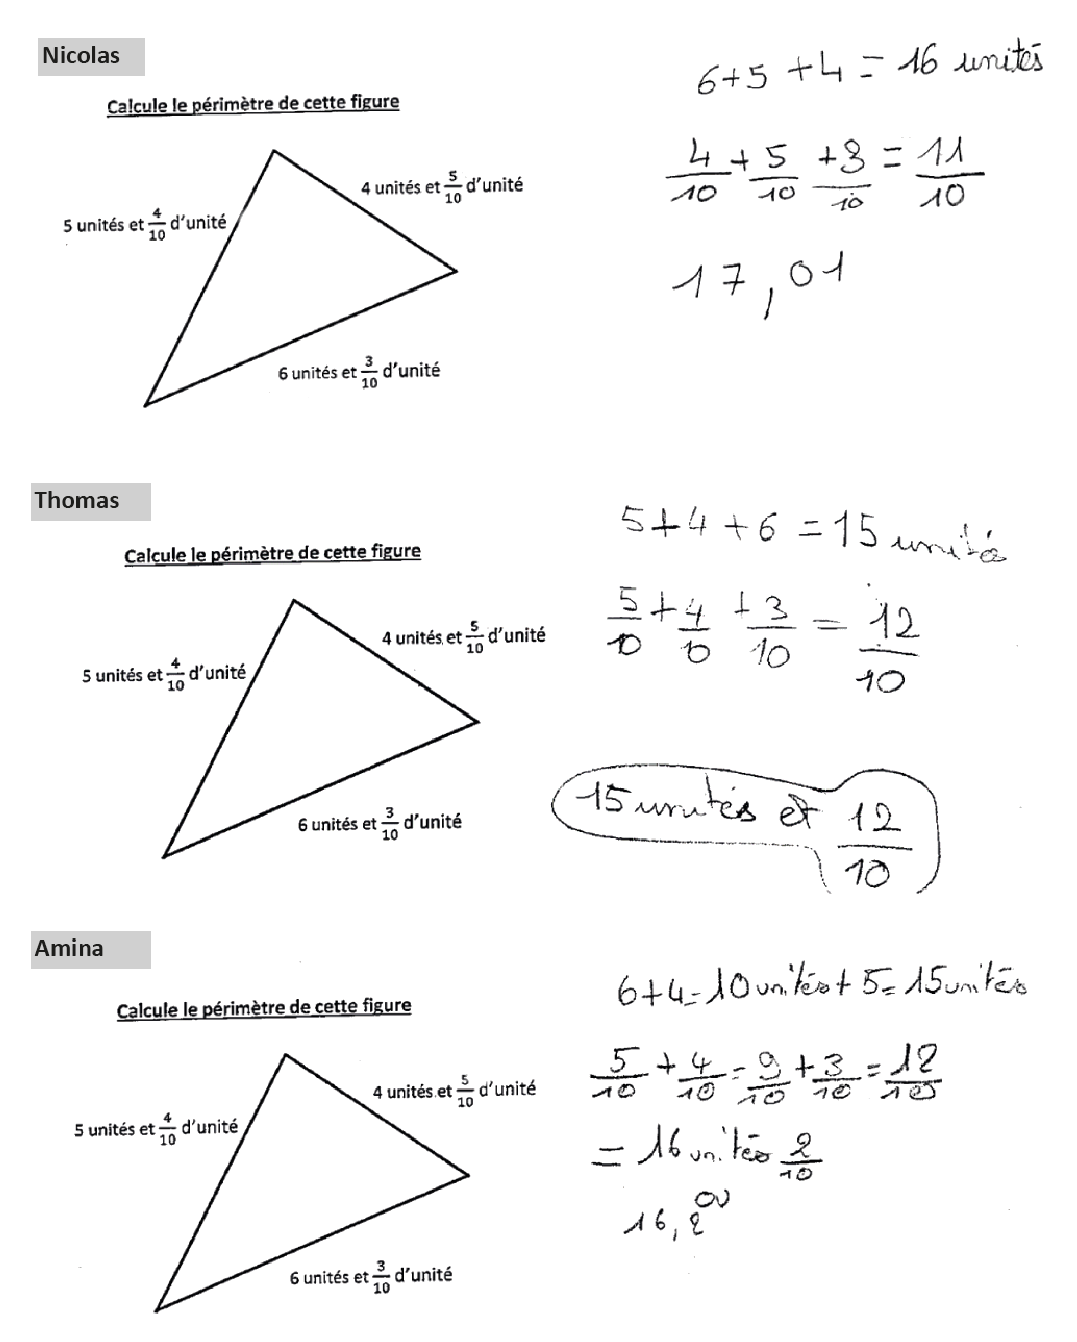
\includegraphics[height=17cm]{Grandeurs_mesures_did/Images/Grm7_analyse_perimetre} \\ [5mm]
   \end{center}
   \item Que peut proposer l’enseignant pour amener Thomas à rédiger sa réponse sous forme d’écriture à virgule ?
\end{enumerate}
\end{exercice}

\begin{corrige}
\ \\ [-5mm]
\begin{enumerate}
   \item {\bf Production de Nicolas.}
   \begin{itemize}
      \item Démarche utilisée : somme des parties entières, somme des parties décimales sous forme de fractions décimales puis transformation en écriture décimale.
      \item Compétence acquise : calcul du périmètre d'un triangle (domaine des grandeurs et mesures).
      \item Erreurs : erreur dans le calcul de la somme des nombres entiers (16 unités au lieu de 15 unités), erreur dans le calcul de la somme des fractions décimales (11 dixièmes au lieu de 12 dixièmes). Erreur de codage : pour 11 dixièmes, il a ajouté une unité et un centième.
   \end{itemize} 
   \smallskip
    {\bf Production de Thomas.}
   \begin{itemize}
       \item Démarche utilisée : somme des parties entières, somme des parties décimales sous forme de fractions décimales puis écriture sous la forme unités et dixièmes.
      \item Compétences acquises : calcul du périmètre d'un triangle (domaine des grandeurs et mesures), somme de nombres entiers et somme de fractions décimales (domaine du calcul).
      \item Erreur : l'écriture n'est pas optimisée, Thomas n'a pas transformé son résultat en une écriture décimale, il n'a pas \og vu \fg{} que 12 dixièmes est égal à une unité et 2 dixièmes.
   \end{itemize}
   \smallskip
   {\bf Production d'Amina.}
   \begin{itemize}
       \item Démarche utilisée : somme des parties entières de proche en proche, somme des parties décimales sous forme de fractions décimales de proche en proche puis écriture sous la forme unités et dixièmes et enfin codage sous forme décimale.
      \item Compétences acquises : calcul du périmètre d'un triangle (domaine des grandeurs et mesures), somme de nombres entiers et somme de fractions décimales (domaine du calcul), codage d'un nombre décimal (domaine des nombres).
      \item Erreur : erreur d'écriture mathématique dans ses sommes (statut du signe égal à revoir).
   \end{itemize}
   \item L'enseignant peut demander à Thomas s'il peut décomposer 12 dixièmes pour l'associer à ses 15 unités, ou lui demander de placer sur une droite graduée son nombre obtenu.
\end{enumerate}
\end{corrige}


%%%%%%%%%
\Recreation %%%
%%%%%%%%%


\setcounter{exercice}{0}
\begin{exercice*}[\fbox{C1} - Comparer et ranger des objets selon leur masse]
Séquence inspirée de {\it Vers les maths MS, Accès}, activité des déménageurs et de la balance. Sauf mention contraire, les séances se font en atelier dirigé. On pourra utiliser l'album \href{https://www.youtube.com/watch?v=Of8ctH03Bx8}{\it Un tout petit coup de main}.
\begin{center}
\begin{tabular}{|p{0.2cm}|p{0.5cm}|p{2.3cm}|p{12.3cm}|}
   \hline
   S & D & Objectif & Déroulement \\
   \hline
   1 &  30 min & Différencier lourd/léger gros/petit &
   {\bf Le jeu des déménageurs} ({\it En classe entière}) \newline
   \uline{Matériel}: des objets de masses et de volumes variés (cartons vides ou pleins, chaises, bancs, ballon, plume, kg de sucre, stylo, bouteille, pack de 6 bouteilles\dots) \newline
   \uline{Déroulement} : transporter les objets d'une zone à l'autre pour imiter des déménageurs. À la fin du jeu, on demande aux élèves de verbaliser ce qu'ils ont fait pour faire émerger le vocabulaire lourd, léger, gros, grand, petit. \\
   \hline
   2 & 30 min & Différencier lourd/léger &
   \uline{Matériel}: les mêmes objets que dans le jeu du déménageur. \newline
   \uline{Déroulement} : classer les objets suivant les deux catégories lourd et léger et valider en énonçant des critères comme \og je peux le porter à une main, à 2 mains, je peux courir avec, j'ai besoin d'un copain pour le porter\dots \fg \\
   \hline
   3 & 10 min & Réinvestissement du vocabulaire lourd/léger &
   {\bf Jeu des devinettes} \newline
   \uline{Matériel}: deux petites bouteilles d'eau, une vide et une pleine et deux grandes bouteilles, une vide et une pleine. \newline
   \uline{Déroulement} : l'enseignant.e choisit une bouteille parmi les quatre et les élèves doivent deviner de laquelle il s'agit en posant des questions. \newline
   Ensuite les élèves peuvent jouer deux par deux. \\
   \hline
   4 & 20 min & Différencier \newline volume/masse &
   \uline{Matériel\textcolor{white}{j}}: des paires d'objet, un grand carton vide fermé, un petit carton fermé rempli d'objets lourds ; une grande bouteille vide et une petite bouteille pleine ; un grand morceau de polystyrène et un petit sac lourd. Chaque objet est marqué d'un signe différent rond ou carré. \newline
   \uline{Déroulement\textcolor{white}{j}}: sans toucher les objets les élèves doivent dire lequel est le plus lourd sans manipuler ni regarder à l'intérieur des objets  en notant le symbole de cet objet. Ensuite ils soupèsent les objets et comparent avec leurs hypothèses. \newline
   Mise en évidence du fait que les plus gros ne sont pas forcément les plus lourds. \\
   \hline
   5 & 30 min & Découverte et \newline manipulation de la balance &
   \uline{Matériel\textcolor{white}{j}}: deux objets de masses voisines . \newline
   \uline{Déroulement\textcolor{white}{j}}: en soupesant les objets les élèves doivent dire lequel des deux est le plus lourd. Les élèves se dessinent en train de soupeser les objets et dictent à l'adulte leur conclusion. Confrontation des résultats et constat des différences. Chercher l'objet de la classe qui pourrait nous aider : la balance. La balance permet de dire quel objet est le plus lourd ou le plus léger. \\
   \hline
   6 & Acc. & Manipulation de la balance &
   Laisser en libre accès la balance au coin jeu pour voir si les enfants l'utilisent pour peser ou plus simplement pour faire faire basculer. \\
   \hline
   7 & 30 min & Réinvestir \newline la balance &
   {\bf Jeu des pirates} \newline
   \uline{Matériel} : quatre coffres (boites) de masses et de couleurs différentes. 
   \newline
   \uline{Déroulement} : distribuer à quatre pirates quatre coffres de masses différentes. Le coffre le plus lourd au capitaine, le coffre un peu moins lourd au matelot, le coffre encore moins lourd au timonier et le coffre le plus léger au mousse. Les coffres sont fermés de même taille mais de couleurs différentes. Les élèves doivent distribuer les coffres aux différents personnages en les pesant à l'aide de la balance. \\
   \hline
\end{tabular}
\end{center}
\end{exercice*}


\begin{exercice*}[\fbox{C2} - Les masses]
   Cette ressource, disponible entièrement ici : \href{http://cache.media.education.gouv.fr/file/Mathematiques/25/8/RA16_C2_MATHS_grandeur_et_mesures_masses_635258.pdf}{Grandeurs et mesures au cycle 2 : masses} est destinée aux élèves de CE1 ou de CE2. \medskip
   
{\bf Objectifs} : utiliser les propriétés additives et multiplicatives des masses pour construire des référents au kilogramme : savoir qu’un kilogramme c’est à peu près la masse d’une bouteille d’un litre d’eau, d’une brique de lait, de cinq pommes, de deux cents feuilles
de papier et donc qu’une ramette de 500 feuilles pèse 2 kilogrammes et demi, etc. Cela permet aussi aux élèves de comprendre qu’à des volumes différents peuvent correspondre des masses identiques et de renforcer la distinction entre masse et contenance/volume. \\
Il convient enfin de faire en sorte que les élèves ne restent pas dans la seule manipulation et entrent dans les références mathématiques (unités de masse, calculs\dots) sans que ce soit l’enseignant qui pose les savoirs (importance de la trace des recherches et de sa formalisation). \medskip

{\bf Matériel} : différents éléments de l’ordre du kilogramme, de tailles, de formes et de compositions variées, issus du quotidien de l’élève ou de la vie courante et mis dans des emballages neutres ; Balance de Roberval et ses masses marquées (sauf 1 kg). \medskip

{\bf Prérequis} : les élèves doivent avoir travaillé en amont sur la grandeur masse et avoir compris de quoi il s’agit. Ils doivent avoir classé des objets selon leur masse, en particulier des objets de masses volumiques différentes afin de bien différencier masse et volume. Une séance préalable d’appropriation et de manipulation des balances de Roberval peut se révéler utile. Il s’agit de faire comprendre aux élèves le principe de l’équilibre. \medskip

{\bf Organisation de la séance} : \\ [1mm]
\begin{tabular}{|p{17cm}|}
   \hline
   Situation 1 : ordonner des objets selon leur masse en les soupesant (15 min) \\
   \hline
   $\bullet$ Présentation et désignation des objets : présenter le contexte de la séance, des objets à peser, les nommer et les lister au tableau. Distribuer les éléments à soupeser. \\
   $\bullet$ Temps de réflexion permettant de préciser le vocabulaire et de recueillir des informations quant aux représentation des élèves. L'enseignant(e) propose la consigne suivante {\it Max dit : \og Toutes ces choses pèsent pareil ! \fg. Lola n’est pas d’accord. Qui a raison ?} \\
   $\bullet$ Recherche en soupesant les objets : les élèves soupèsent les éléments (trois par groupe) et les ordonnent en fonction de leur masse. À l’issue de la séance, ils gardent une trace écrite (photographie, courte phrase, ordre de vignettes\dots). \\
   \hline
\end{tabular}

\smallskip

\begin{tabular}{|p{17cm}|}
   \hline
   Situation 2 : ordonner des objets selon leur masse par comparaison et pesée (15 min) \\
   \hline
   $\bullet$ Recherche par comparaison deux à deux. L'enseignant(e) propose la consigne suivante : {\it Pour vérifier la classification que vous avez établie, vous allez utiliser les balances pour comparer les objets deux à deux}. \\
   Les élèves comparent les masses des objets en les déposant sur les plateaux de la balance Roberval. Ils sont invités à rédiger une phrase de conclusion. \\
   $\bullet$ Recherche par pesée. L'enseignant(e) propose la consigne suivante : {\it Déterminer la masse de chacun des objets à l’aide de la balance et des masses marquées}. Distribuer des masses marquées (la somme de ces masses doit faire au moins un kilogramme). Faire réaliser une mesure pour chacun des objets. \\
   \hline
\end{tabular}

\smallskip

\begin{tabular}{|p{17cm}|}
   \hline
   Situation 3 : construction de référents de l’ordre du kilogramme (15 min) \\
   \hline
   $\bullet$ Un tableau récapitulatif permet de faire la synthèse des différentes pesées effectuées en notant les résultats. Si plusieurs groupes ont pesé les mêmes objets, on peut faire apparaitre les différentes mesures obtenues. Ces différentes mesures ne seront sans doute pas égales, il faut alors différencier les résultats incohérents dus à des erreurs de lecture des masses ou de calcul des différences, des résultats simplement différents à cause de l’incertitude de la mesure (comment les objets sont placés sur le plateau, type d’arrondi, etc.). \\
   $\bullet$ Élaboration de la trace écrite : faire émerger la notion de référent au kilogramme. \\
   \hline
\end{tabular}

\end{exercice*}


\begin{exercice*}[\fbox{C2/C3} - Le goûter]
   Cette ressource issue d'{\itéduSCOL} propose une activité qui s’appuie sur un projet de goûter pour une association sportive. Elle permet de travailler en mathématiques, dans le domaine \og Grandeurs et mesures \fg, les principes d’utilisation de la monnaie et le lexique associé ainsi que la résolution de problèmes. \\
   Le scénario pédagogique décline cette activité selon cinq niveaux de progressivité aux cycles 2 et 3. La situation proposée se complexifie progressivement, en jouant sur les variables didactiques. L’activité consiste en la résolution d’un problème dont l’énoncé est volontairement épuré et schématisé. À partir de cette situation initiale, les évolutions proposées permettent à l’enseignant de prendre en compte l’hétérogénéité de la classe. \\ [4mm]
   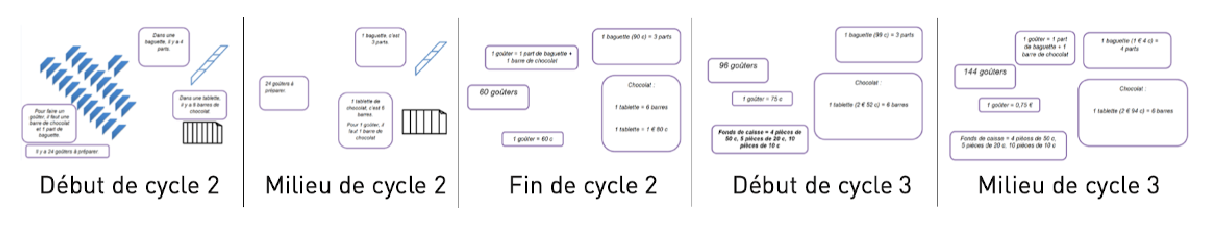
\includegraphics[width=17cm]{Grandeurs_mesures_did/Images/Grm7_activite_gouters} \\ [2mm]
{\bf Présentation de la situation aux élèves} : \\
\og Dans une association sportive, des enfants proposent un goûter payant à l’ensemble des adhérents. Ce goûter est constitué d’une part de baguette de pain et d’une barre de chocolat. Afin de prévoir les goûters, l’un des enfants organisateurs a représenté la situation par un schéma. \fg

{\bf Organisation} :
\begin{itemize}
   \item prévoir un temps de recherche préalable autour du document en collectif, par binôme ou en petit groupe à partir d’une série non exclusive de questions : \og Qu’est-ce que l’enfant a écrit et dessiné sur son schéma ? \fg, \og A quoi cela peut-il bien lui servir ? \fg, \og En quoi cela est-il utile ? \fg, \og Que va-t-il bien pouvoir en faire ? \fg\dots
   \item mise en commun avec validation des hypothèses.
   \item l’enseignant.e introduit ensuite des données financières de la situation de référence : le goûter est vendu\dots, la baguette coûte\dots, la tablette de chocolat coûte\dots{} puis il pose la question suivante : \\
   \og Que pouvez-vous calculer à partir de ces données ? Effectuer les calculs qui permettent de connaître les recettes et les dépenses. Les recettes couvrent-elles les dépenses ? \fg
   \item les élèves rendent un écrit. \\
\end{itemize}


\begin{minipage}{7cm}
   {\bf Niveau 1 : début de cycle 2} \\ [3mm]
   \uline{Prérequis} : savoir que 50 c + 50 c = \ueuro{1} \\ [3mm]
   \uline{Données financières} : \\
   le goûter est vendu 50 c, \\
   la baguette coûte \ueuro{1}, \\
   la tablette de chocolat coûte \ueuro{2}.
\end{minipage}
\begin{minipage}{8cm}   
   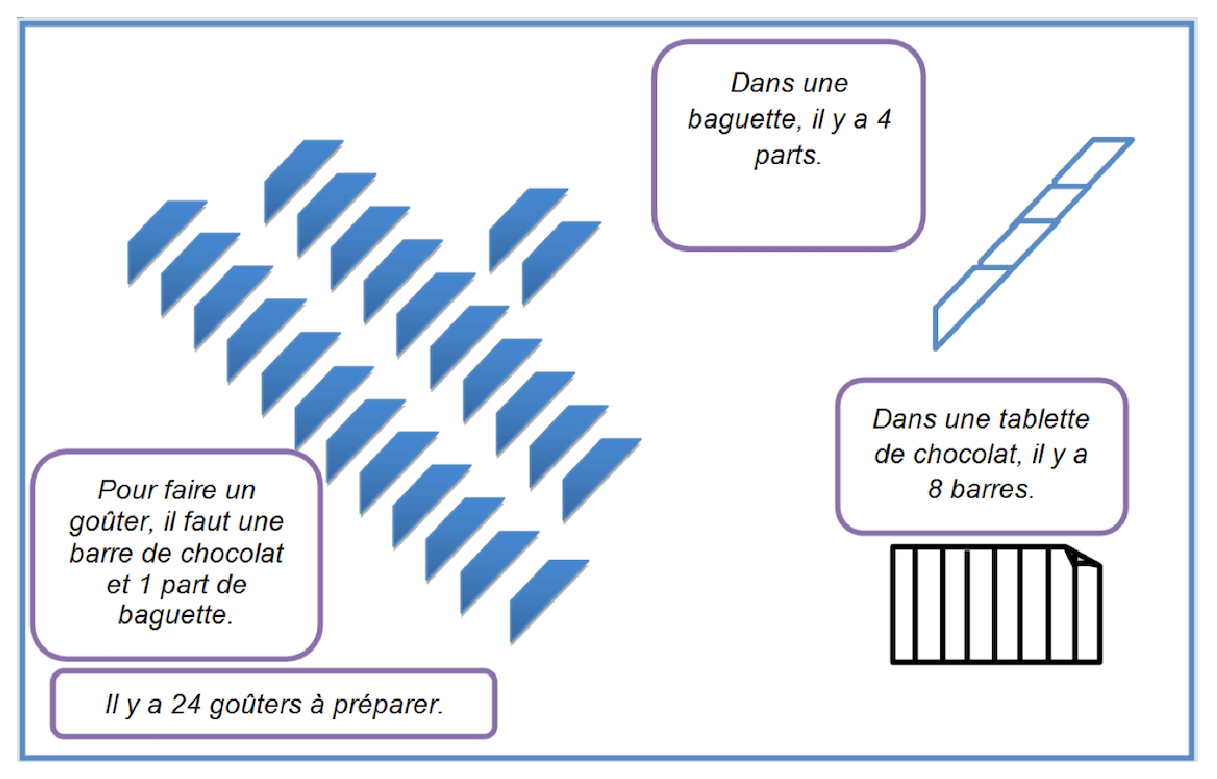
\includegraphics[width=10cm]{Grandeurs_mesures_did/Images/Grm7_activite_gouter1}
\end{minipage}

\begin{minipage}[t]{8cm}
   {\bf Niveau 2 : milieu de cycle 2} \\ [2mm]
   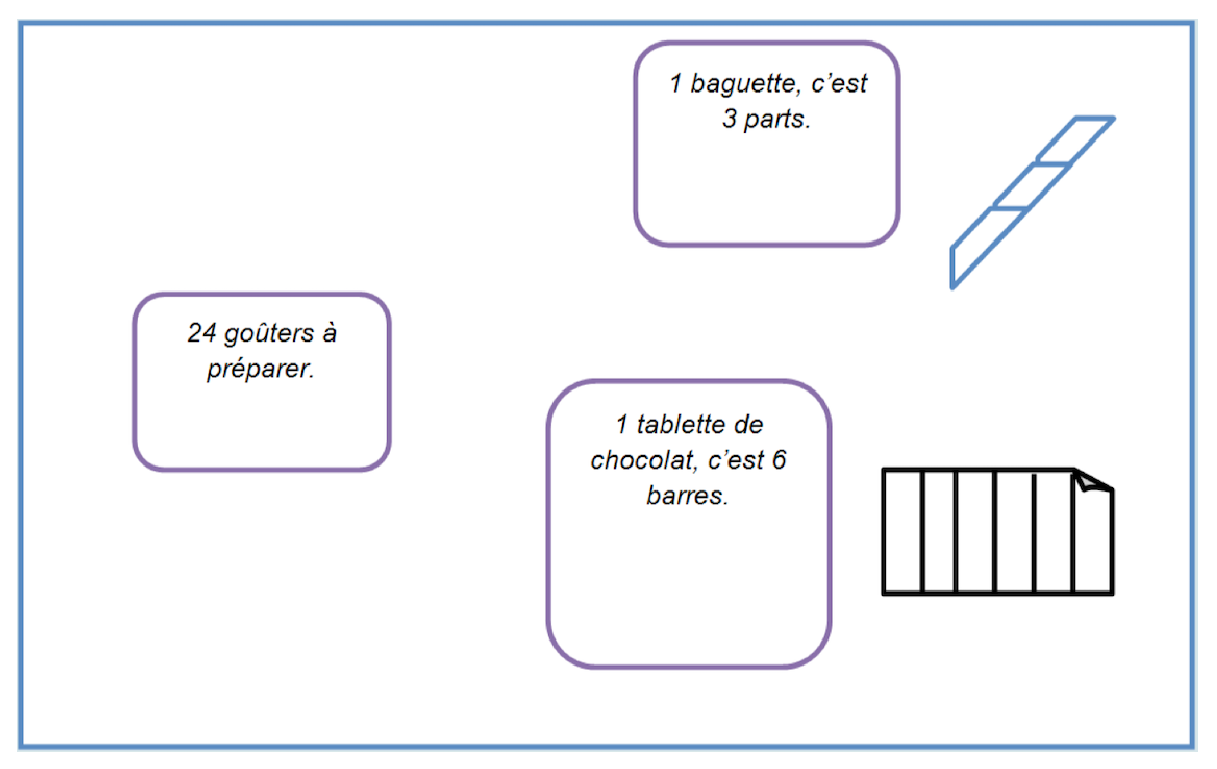
\includegraphics[height=5cm]{Grandeurs_mesures_did/Images/Grm7_activite_gouter2} \\
   \uline{Prérequis} : manipuler les centimes d'euro \\
   par tranches de 25 c \\ [2mm] 
   \uline{Données financières} : \\
   le goûter est vendu 75 c, \\
   la baguette coûte \ueuro{1,25}, \\
   la tablette de chocolat coûte \ueuro{2}.
\end{minipage}
\begin{minipage}[t]{8cm}
      {\bf Niveau 3 : fin de cycle 2} \\ [2mm]
      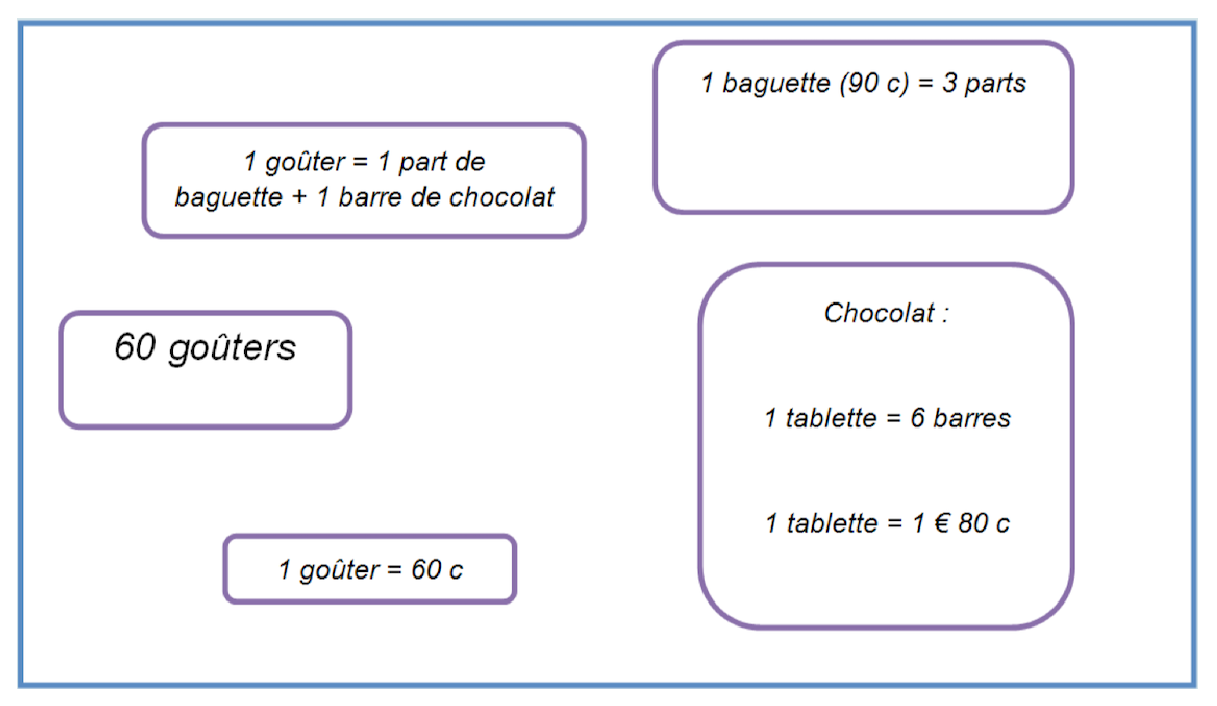
\includegraphics[height=5cm]{Grandeurs_mesures_did/Images/Grm7_activite_gouter3} \\
   \uline{Données financières} : \\
   données sur le schéma.
\end{minipage}

\ \\ [4mm]

\begin{minipage}[t]{8cm}
   {\bf Niveau 4 : début de cycle 3} \\ [2mm]
   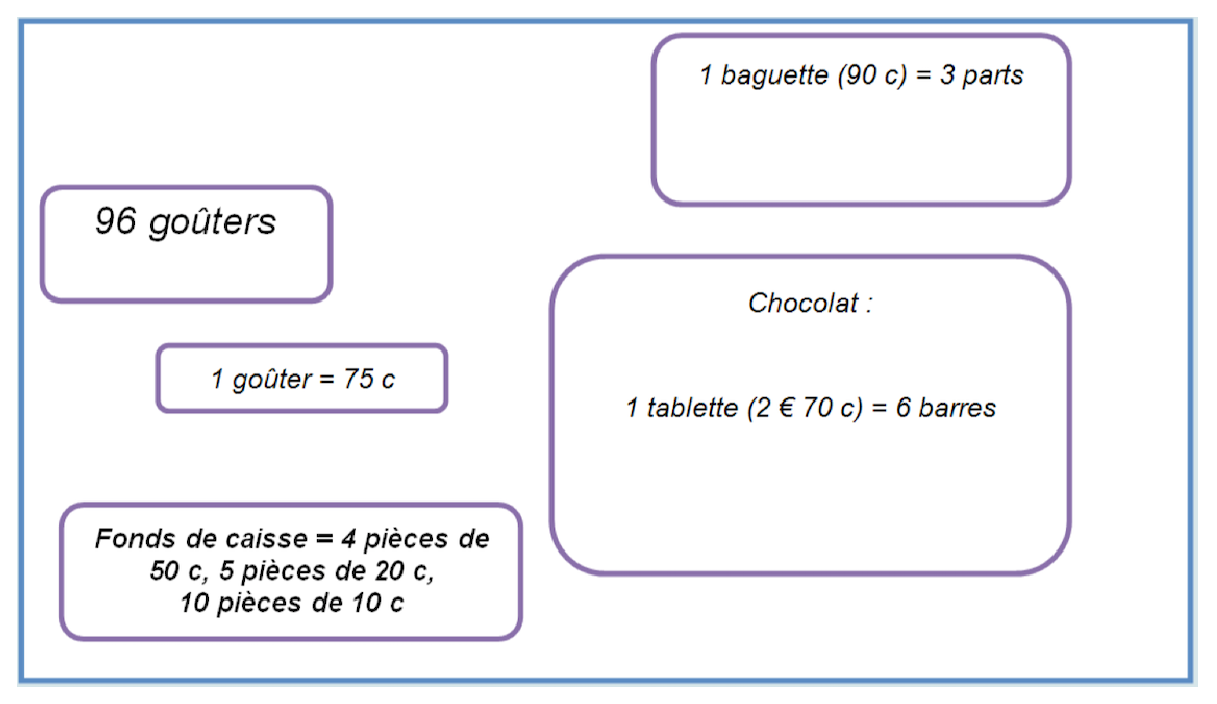
\includegraphics[height=4.9cm]{Grandeurs_mesures_did/Images/Grm7_activite_gouter4} \\
   \uline{Contenu de la caisse après la vente} : \\
      39 pièces de \ueuro{1}, \\
      52 pièces de 50 c \\
      25 pièces de 20 c \\
      49 pièces de 10 c \\
      22 pièces de 5 c 
\end{minipage}
\begin{minipage}[t]{8cm}
   {\bf Niveau 5 : fin de cycle 3} \\ [2mm]
   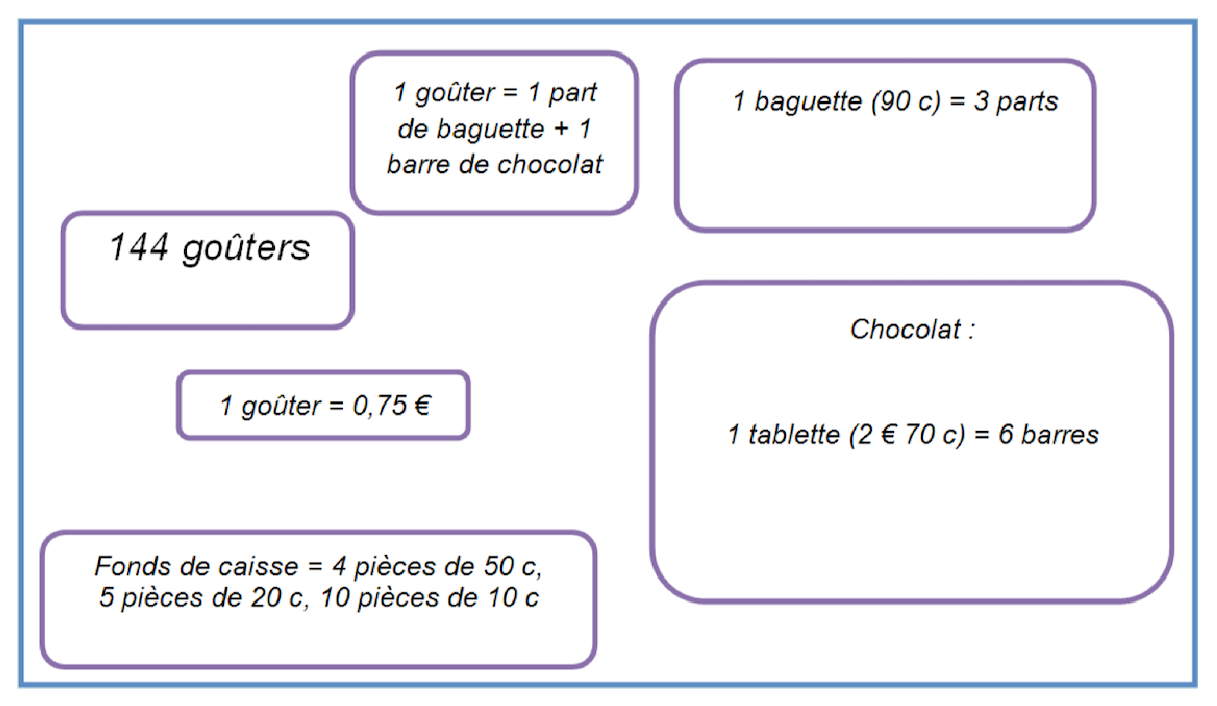
\includegraphics[height=4.9cm]{Grandeurs_mesures_did/Images/Grm7_activite_gouter5} \\
   \uline{Contenu de la caisse après la vente} : \\
      5 billets de \ueuro{5} \\
   16 pièces de \ueuro{2} \\
   35 pièces de \ueuro{1} \\  
   31 pièces de 50 c \\
   10 pièces de 20 c \\
   11 pièces de 10 c \\
   18 pièces de 5 c \\
   21 pièces de 2 c \\
   8 pièces de 1 c
\end{minipage}

\end{exercice*}

